\chapter{Experiments design and results}
\label{chap:expe}
\textit{In this Chapter I expose all details about the evaluation process of \posl{}, i.e., all experiments I perform. For each benchmark, I explain used strategies in the evaluation process and the used environments were the runs were performed (\textit{Curiosiphi} server). %, and eventually \textit{Grid5000}). 
I describe all the experiments and I expose a complete analysis of the obtained result.}
\vfill
\minitoc
\newpage

In this chapter I illustrate and analyze the versatility of \posl{} studying different ways to solve constraint problems based on local search meta-heuristics. 
I have chosen the \sgp, the \nqp, the \carrp{} and the \grp{} as benchmarks since they are challenging yet differently structured problems. In this Chapter I present formally each benchmark, I explain the structure of \posl's solvers that I have generated for experiments and present a detailed analysis of obtained results.

The experiments\footnote{\posl{} source code is available on GitHub:\href{https://github.com/alejandro-reyesamaro/POSL}{https://github.com/alejandro-reyesamaro/POSL}} 
were performed on an Intel\R{} Xeon\TM{} E5-2680 v2, 10$\times$4 cores, 2.80GHz. This server is called \textit{Coriosiphi} and is located at \textit{Laboratoire d'Informatique de Nantes Atlantique}, at the Universiti of Nantes. Showed results are the means of 30 runs for each setup, presented in columns labeled {\bf T}, corresponding to the run-time in seconds, and {\bf It.} corresponding to the number of iterations; and their respective standard deviations ({\bf T(sd)} and {\bf It.(sd)}). In some tables, the column labeled \textbf{\% success} indicates the percentage of solvers finding a solution before reaching a time--out (5 minutes).

\modified{The experiments in this Chapter are multi-walk runs}. Parallel experiments use 40 cores for all problem instances. It is important to point out that \posl{} is not designed to obtain the best results in terms of performance, but to give the possibility of rapidly prototyping and studying different cooperative or non cooperative search strategies.

\modified{All benchmarks were coded using the \posl{} low-level framework in C++.}

\modified{First results using \posl{} to solve} constraint problems were published in \cite{Reyes-amaro} were we used \posl{} to solve the \sgp{} and study some communication strategies. It was the first version of \posl{}, therefore it was able to solve only relatively easy instances. However, the efficacy of the communication was showed using this tool.

\modified{With the next and more optimized version of \posl{}, I decide to start to perform more detailed studies using the benchmark mentioned before and some others.}

\section{Solving the \sgp}
\label{sec:golfers}

In this section I present the performed study using \sgp{} (\SGP) as a benchmark. The \commstr{} analyzed here consists in applying a mechanism of cost descending acceleration, exchanging the current configuration between two solvers with different characteristics. Final obtained results show that this \commstr{} works pretty well for this problem.

\subsection{Problem definition}

The \sgp{} (\SGP) consists in scheduling $g\times p$ golfers into $g$ groups of $p$ players every week for $w$ weeks, such that two players play in the same group at most once. An instance of this problem can be represented by the triple $g-p-w$. This problem, and other closely related problems, arise in many practical applications such as encoding, encryption, and covering problems~\cite{Lardeux2014}. Its structure is very attractive, because it is very similar to other problems, like \textit{Kirkman's Schoolgirl Problem} and the \textit{Steiner Triple System}. %, so efficient modules to solve a broad range of problems can be built.

The cost function for this benchmark was implemented making an efficient use of the stored information about the cost of the previews configuration. Using integers to work with bit-flags, a table to store the information about the partners of each player in each week can be filled in $O\left(p^2\cdot g \cdot w\right)$. So, if a configuration has $n = (p\cdot g \cdot w)$ elements, this table can be filled in $O\left(p\cdot n\right)$. This table is filled from scratch only one time in the search process (I explain in the next section why). Then, every cost of a new configuration, is calculated based on this information and the performed changes between the new configuration and the stored one. This relative cost is calculated in $O\left(c\cdot g\right)$, where $c$ is the number of performed changed in the new configuration with respect to the stored one.

\subsection{Experiment design and results}

Here, I present the \as{} designed for this problem as well as concrete \oms{} composing the different solvers I have tested:

\begin{enumerate}
	\item Generation abstract module $I$:
	\subitem $I_{BP}$: Returns a random configuration $s$, respecting the structure of the problem, {\it i.e.}, the configuration is a set of $w$ permutations of the vector $[1..n]$, where $n=g\times p$.
	\item Neighborhood abstract modules $V$:
	\subitem $V_{std}$: Given a configuration, returns the neighborhood $\mathcal{V}\left(s\right)$ swapping players among groups.
	\subitem $V_{BAS}$: Given a configuration, returns the neighborhood $\mathcal{V}\left(s\right)$ swapping the most culprit player with other players from the same week. It is based on the {\it Adaptive Search} algorithm.
	\subitem $V_{BP}(p)$: Given a configuration, returns the neighborhood $\mathcal{V}\left(s\right)$ by swapping the most culprit player with other players in the same week, for all $p$ randomly selected weeks.
	\item Selection abstract modules $S$:
	\subitem $S_{first}$: Given a neighborhood, selects the first configuration $s' \in V\left(s\right)$ improving the current cost and returns it together with the current one into the pair $\left(s', s\right)$.
	\subitem $S_{best}$: Given a neighborhood, selects the best configuration $s' \in V\left(s\right)$ improving the current cost and returns it together with the current one into the pair $\left(s', s\right)$.
	\subitem $S_{rand}$: Given a neighborhood, selects randomly a configuration $s' \in V\left(s\right)$ and returns it together with the current one, into the pair $\left(s', s\right)$.
	\item Acceptance abstract module $A$:
	\subitem $A_{AI}$: Given a pair $\left(s', s\right)$, returns always the configuration $s'$
\end{enumerate}

These concrete modules are very useful and can be reused to solve tournament-like problems like \textit{Sports Tournament Scheduling}, \textit{Kirkman's Schoolgirl} and the \textit{Steiner Triple System} problems.

In a first stage of the experiments I use the operator-based language provided by \posl{} to build and test many different non communicating strategies. The goal is to select the best concrete modules to run tests performing communication. A very first experiment was performed to select the best neighborhood function to solve the problem, comparing a basic solver using $V_{std}$; a new solver using $V_{BAS}$; and a combination of $V_{std}$ and $V_{BAS}$ by applying the operator $\circled{$\rho$}$, already introduced in the previous chapter. Algorithms~\ref{as:golfers10-10-3} and \ref{as:golfers_rho} present solvers for each case, respectively.

\begin{algorithm}[t]
\dontprintsemicolon
\SetNoline
\SetKwProg{myproc}{\tet{\bf abstract solver}}{\tet{\bf begin}}{\tet{\bf end}}
\myproc{as\_simple \tcp*{{\sc Itr} $\rightarrow$ number of iterations}
	\tet{\bf computation} : $I, V, S, A$\;}{
	\whileinline{$\left(\textbf{\Iter < } K_1\right)$}{%M_1^a \circled{$\rho$} M_1^b
		$I \poslop{\mapsto}$
		\whileinline{$\left(\textbf{\Iter \% } K_2\right)$}{$\left[V \poslop{\mapsto} S \poslop{\mapsto} A\right]$}
	}	
}
\tet{\bf solver} \solverposl{Std} \tet{\bf implements} as\_simple\;
\algoindent \tet{\bf computation} : $I_{BP}, V_{std}, S_{best}, A_{AI}$ \;
\tet{\bf solver} \solverposl{AS} \tet{\bf implements} as\_simple\;
\algoindent \tet{\bf computation} : $I_{BP}, V_{BAS}, S_{best}, A_{AI}$ \; 
%\tet{\bf connection}: $CM_{last}$\;
\caption{Simple solvers for \SGP}\label{as:golfers10-10-3}
\end{algorithm}

\begin{algorithm}[H]
\dontprintsemicolon
\SetNoline
\SetKwProg{myproc}{\tet{\bf abstract solver}}{\tet{\bf begin}}{\tet{\bf end}}
\myproc{as\_rho \tcp*{{\sc Itr} $\rightarrow$ number of iterations}
	\tet{\bf computation} : $I, V_1, V_2, S, A$\;}{
	\whileinline{$\left(\textbf{\Iter < } K_1\right)$}{%M_1^a \circled{$\rho$} M_1^b
		$I \poslop{\mapsto}$
		\whileinline{$\left(\textbf{\Iter \% } K_2\right)$}{$\left[\left[V_1 \poslop{\rho} V_2\right] \poslop{\mapsto} S \poslop{\mapsto} A\right]$}
	}	
}
\tet{\bf solver} \solverposl{rho} \tet{\bf implements} as\_rho\;
\algoindent \tet{\bf computation} : $I_{BP}, V_{std}, V_{BAS}, S_{best}, A_{AI}$ \;
\caption{Solvers combining neighborhood functions using operator {\it RHO}}\label{as:golfers_rho}
\end{algorithm}

\begin{table}
\centering 
\renewcommand{\arraystretch}{1}
\begin{tabular}{p{4cm}|R{1.3cm}R{1.3cm}R{1.3cm}R{1.3cm}}
\hline
{\bf Solver} & T & T(sd) & It. & It.(sd) \\
\hline
%\hline
\texttt{\solverposl{AS}} & \good{\bf 1.06} & 0.79 & 352 & 268 \\		
\texttt{\solverposl{rho}} & 41.53 & 26.00 & 147 & 72\\
%Std $\circled{$\cup$}$ AS & 59.65 & 55.01 & 198 & 110\\
\texttt{\solverposl{Std}} & 87.90 & 41.96 & 146 & 58 \\
\hline
\end{tabular}
\caption{\sg: Instance 10--10--3 in parallel}
\label{tab:golfers10-10-3}
\end{table}

Results in Table~\ref{tab:golfers10-10-3} are not surprising. The neighborhood module $V_{BAS}$ is based on the {\it Adaptive Search} algorithm, which has shown very good results \cite{Diaz}. %It selects the variable (player) contributing the most to the cost and permutes its value with the others variables (players) for all groups, every week.
It selects the most culprit variable (i.e., a player), that is, the variable the most responsible for constraints violation. Then, it permutes this variable value with the value of each other variable, in all groups and all weeks. Each permutation gives a neighbor of the current configuration. $V_{Std}$ uses no additional information, so it performs every possible swap between two players in different groups, every week. It means that this neighborhood is $g\times p$ times bigger than the previous one, with $g$ the number of groups and $p$ the number of players per group. 
It allows for more organized search because the set of neighbors is pseudo-deterministic, i.e., the construction criteria is always the same but the order of the configuration is random. On the other hand, {\it Adaptive Search} neighborhood function takes random decisions more frequently, and the order of the configurations is random as well. We also tested a solver with combining these modules using the $\circled{$\rho$}$ operators. This operator executes its first or second parameter depending on a given probability $\rho$. This combination spent more time searching the best configuration among the neighborhood, although with a lower number of iterations than $V_{BAS}$. The $V_{BAS}$ neighborhood function being clearly faster, we have chosen it for our experiments, even if it shown a more spread standard deviation: 0.75 for \solverposl{AS} versus 0.62 for \solverposl{Std}, considering the ratio $\tfrac{T(sd)}{T}$.

\separation

Once the neighborhood \om{} has been selected, I have focused the experiment on choosing the best {\it selection} \om. Solvers mentioned above were too slow to solve instances of the problem with more than three weeks: they were very often trapped into local minima. For that reason, another solver implementing the \as{} described in Algorithm~\ref{as:golfers_b001} have been created, using $V_{BAS}$ and combining $S_{best}$ and $S_{rand}$: it tries a number of times to improve the cost, and if it is not possible, it picks a random neighbor for the next iteration. We also compared the $S_{first}$ and $S_{best}$ selection modules. The \om{} $S_{best}$ selects the best configuration inside the neighborhood. It did not only spend more time searching a better configuration, but also is was more sensitive to become trapped into local minima. The second \om{} $S_{first}$ selects the first configuration inside the neighborhood improving the current cost. Using this module, solvers favor exploration over intensification and of course spend clearly less time searching into the neighborhood. 

\begin{algorithm}[H]
\dontprintsemicolon
\SetNoline
\SetKwProg{myproc}{\tet{\bf abstract solver}}{\tet{\bf begin}}{\tet{\bf end}}
\myproc{as\_eager \tcp*{{\sc Itr} $\rightarrow$ number of iterations}
	\tet{\bf computation} : $I, V, S_1, S_2, A$\;}{
	\whileinline{$\left(\textbf{\Iter < } K_1\right)$}{%M_1^a \circled{$\rho$} M_1^b
		$I \poslop{\mapsto}$
		\whileinline{$\left(\textbf{\Iter \% } K_2\right)$}{$\left[V \poslop{\mapsto} \left[S_1 \poslopcond{\Sci < K_3} S_2\right] \poslop{\mapsto} A\right]$}
	}
}
\tet{\bf solver} \solverposl{best} \tet{\bf implements} as\_eager\;
\algoindent \tet{\bf computation} : $I_{BP}, V_{std}, V_{BAS}, S_{best}, S_{rand}, A_{AI}$ \;
\tet{\bf solver} \solverposl{first} \tet{\bf implements} as\_eager\;
\algoindent \tet{\bf computation} : $I_{BP}, V_{std}, V_{BAS}, S_{first}, S_{rand}, A_{AI}$ \;
\caption{Solver for \SGP{} to scape from local minima}\label{as:golfers_b001}
\end{algorithm}

\begin{table}
\captionsetup{belowskip=6pt,aboveskip=6pt}
\centering 
\renewcommand{\arraystretch}{1}
\begin{tabular}{p{2cm}|R{1cm}R{1cm}R{1cm}R{1.2cm}|R{1cm}R{1cm}R{1cm}R{1.2cm}}
	\hline %\noalign{\smallskip}	
	\multirow{2}{*}{\footnotesize{\centering {\bf Instance}}} & 
	\multicolumn{4}{c|}{Best improvement} & 
	\multicolumn{4}{c}{First improvement}\\
	\cline{2-9} %\cline{3-8}
	& T & T(sd) & It. & It.(sd) & T & T(sd) & It. & It.(sd) \\
	\hline
	%\hline
	5--3--7 & 0.45 & 0.70 & 406 & 726 & 0.23 & 0.14 & 142 & 67\\
	8--4--7 & 0.37 & 0.11 & 68 & 13 & 0.28 & 0.07 & 93 & 13\\	
	9--4--8 & 0.87 & 0.13 & 95 & 17 & 0.60 & 0.16 & 139 & 18 \\
	\hline
\end{tabular}
\caption{\sg: comparing selection functions in parallel}
\label{tab:golfersB001}
\end{table}

\begin{table}[h]
\centering
\renewcommand{\arraystretch}{1}
\begin{tabular}{p{1.5cm}|R{1.5cm}R{1.5cm}R{1.5cm}R{1.5cm}}
\hline
{\bf Instance} & T & T(sd) & It. & It.(sd)\\
\hline
%\hline
5--3--7 & 1.25 & 1.05 & 2,907 & 2,414 \\
8--4--7 & 0.60 & 0.33 & 338 & 171 \\
9--4--8 & 1.04 & 0.72 & 346 & 193\\
\hline
\end{tabular}
\caption{\sg: a single sequential solver using first improvement}
\label{tab:golfers_seq}
\end{table}

Tables~\ref{tab:golfersB001} and \ref{tab:golfers_seq} present results of this experiment, showing that a local exploration-oriented strategy is better for the \SGP. If we compare results of Tables~\ref{tab:golfersB001} \ref{tab:golfers_seq} with respect to the standard deviation, we can some gains in robustness with parallelism. The spread in the running times and iterations for the instance 5--3--7 is 24\% lower (0.84 sequentially versus 0.60 in parallel), for 8--4--7 is 30\% lower (0.55 sequentially versus 0.25 in parallel) and for 9--4--8 (the hardest one) is 43\% lower (0.69 sequentially versus 0.26 in parallel), using the same ratio $\tfrac{T(sd)}{T}$).

\separation

The conclusion of the last experiment was that the best solver to solve \SGP{} using \posl{} is the one using a neighborhood \om{} based on {\it Adaptive Search} algorithm ($V_{BAS}$) and a selection \om{} selecting the first configuration improving the cost. Using this solver as a base, the next step was to design a simple communication strategy where the shared information is the current configuration. Algorithms~\ref{as:golfers_sender}~and~\ref{as:golfers_receiver} show that the communication is performed while applying the acceptance criterion of the new configuration for the next iteration. Here, receiver solvers receive a configuration from a sender solver, and match it with their current configuration. Then, the configuration with the lowest global cost is selected. This operation is coded using the \textit{minimum} operator $\poslop{m}$ in Algorithm~\ref{as:golfers_receiver}. This way, the receiver solver continues the search from a more promising place into de search space. Different communication strategies were designed, either executing a full connected solvers set, or a tuned combination of connected and unconnected solvers. Between connected solvers, two different connections operations were applied: connecting each sender solver with one receiver solver (\oneTone), or connecting each sender solver with all receiver solvers (\oneTn). The code for the different \commstrs{} are presented in Algorithms~\ref{comm:golfers_1_1-1} to \ref{comm:golfers_1_1-n_25}.

\begin{algorithm}
\dontprintsemicolon
\SetNoline
\SetKwProg{myproc}{\tet{\bf abstract solver}}{\tet{\bf begin}}{\tet{\bf end}}
\myproc{as\_eager\_sender \tcp*{{\sc Itr} $\rightarrow$ number of iterations}
	\tet{\bf computation} : $I, V, S_1, S_2, A$\tcp*{{\sc Sci} $\rightarrow$ number of iterations with the same cost}}{%	
	\whileinline{$\left(\textbf{\Iter < } K_1\right)$}{
		$I \poslop{\mapsto}$
		\whileinline{$\left(\textbf{\Iter \% } K_2\right)$}{$\left[V \poslop{\mapsto} \left[S_1 \poslopcond{\Sci < K_3} S_2\right] \poslop{\mapsto} \llparenthesis A \rrparenthesis^o\right]$}
	}
}
\tet{\bf solver} \solverposl{sender} \tet{\bf implements} as\_eager\_sender\;
\algoindent \tet{\bf computation} : $I_{BP}, V_{BAS}, S_{first}, S_{rand}, A_{AI}$ \;
\caption{Communicating \as{} for \SGP{} (sender)}\label{as:golfers_sender}
\end{algorithm}

\begin{algorithm}
\dontprintsemicolon
\SetNoline
\SetKwProg{myproc}{\tet{\bf abstract solver}}{\tet{\bf begin}}{\tet{\bf end}}
\myproc{as\_eager\_receiver \tcp*{{\sc Itr} $\rightarrow$ number of iterations}
	\tet{\bf computation} : $I, V, S_1, S_2, A$\tcp*{{\sc Sci} $\rightarrow$ number of iterations with the same cost}
	\tet{\bf communication} : $C.M.$\;}{%	
	\While{$\left(\textbf{\Iter < } K_1\right)$}{%M_1^a \circled{$\rho$} M_1^b
		$I \poslop{\mapsto}$
		\whileinline{$\left(\textbf{\Iter \% } K_2\right)$}{
			$ V \poslop{\mapsto} \left[S_1 \poslopcond{\Sci < K_3} S_2\right] \poslop{\mapsto} \left[A \poslop{m} C.M.\right]$
		}
	}
}
\tet{\bf solver} \solverposl{receiver} \tet{\bf implements} as\_eager\_receiver\;
\algoindent \tet{\bf computation} : $I_{BP}, V_{BAS}, S_{first}, S_{rand}, A_{AI}$ \;
\algoindent \tet{\bf communication} : $CM_{last}$
\caption{Communicating \as{} for \SGP{} (receiver)}\label{as:golfers_receiver}
\end{algorithm}

\begin{algorithm}
\dontprintsemicolon
\SetNoline
$\left[\eqsolverposl{sender}\cdot A\right] \onetoone \left[\eqsolverposl{receiver}\cdot C.M.\right]20;$
\caption{Communication strategy \oneTone{} 100\%}\label{comm:golfers_1_1-1}
\end{algorithm}

\begin{algorithm}
\dontprintsemicolon
\SetNoline
$\left[\eqsolverposl{sender}\cdot A(20)\right] \oneton \left[\eqsolverposl{receiver}\cdot C.M.(20)\right];$
\caption{Communication strategy \oneTn{} 100\%}\label{comm:golfers_1_1-n}
\end{algorithm}

\begin{algorithm}
\dontprintsemicolon
\SetNoline
$\left[\eqsolverposl{sender}\cdot A\right] \onetoone \left[\eqsolverposl{receiver}\cdot C.M.\right]10;$\;
$\left[\eqsolverposl{first}\right]20;$
\caption{Communication strategy \oneTone{} 50\%}\label{comm:golfers_1_1-1_50}
\end{algorithm}

\begin{algorithm}
\dontprintsemicolon
\SetNoline
$\left[\eqsolverposl{sender}\cdot A(10)\right] \oneton \left[\eqsolverposl{receiver}\cdot C.M.(10)\right];$\;
$\left[\eqsolverposl{first}\right]20;$
\caption{Communication strategy \oneTn{} 50\%}\label{comm:golfers_1_1-n_50}
\end{algorithm}

\begin{algorithm}
\dontprintsemicolon
\SetNoline
$\left[\eqsolverposl{sender}\cdot A\right] \onetoone \left[\eqsolverposl{receiver}\cdot C.M.\right]5;$\;
$\left[\eqsolverposl{first}\right]30;$
\caption{Communication strategy \oneTone{} 25\%}\label{comm:golfers_1_1-1_25}
\end{algorithm}

\begin{algorithm}
\dontprintsemicolon
\SetNoline
$\left[\eqsolverposl{sender}\cdot A(5)\right] \oneton \left[\eqsolverposl{receiver}\cdot C.M.(5)\right];$\;
$\left[\eqsolverposl{first}\right]30;$
\caption{Communication strategy \oneTn{} 25\%}\label{comm:golfers_1_1-n_25}
\end{algorithm}

In Algorithm~\ref{as:golfers_receiver}, the abstract \opch{} $C.M.$ was instantiated with the concrete \opch{} $CM_{last}$, which takes into account the last received configuration at the time of its execution.

Each time a \posl{} meta-solver is launched, many independent search solvers are executed. We call "good" configuration a configuration with the lowest cost within the current configuration neighborhood and with a cost strictly lesser than the current one. Once a good configuration is found in a sender solver, it is transmitted to the receiver one. At this moment, if the information is accepted, there are some solvers searching in the same subset of the search space, and the search process becomes more exploitation--oriented. This can be problematic if this process makes solvers converging too often towards local minima. In that case, we waste more than one solver trapped into a local minima: we waste all solvers that have been attracted to this part of the search space because of communications. This phenomenon is avoided through a simple (but effective) play: if a solver is not able to find a better configuration inside the neighborhood (executing $S_{first}$), it selects a random one at the next iteration (executing $S_{rand}$).

In all Algorithms in this section, three parameter can be found:\begin{inparaenum}[1.] \item $K_1$: the maximum number of {\it restarts}, \item $K_2$: the maximum number of iterations in each \textit{restart}, and $K_3$: the maximum number of iterations with the same current cost. \item \end{inparaenum}

After the selection of the proper modules to study different communication strategies, I proceeded to tune these parameter. Only a few runs were necessaries to conclude that the mechanism of using the \om{} $S_{rand}$ to scape from local minima was enough. For that reason, since the solver never perform restarts, the parameter $K_1$ was irrelevant. So the reader can assume $K_1 = 1$ for every experiment.

With the certainty that solvers do not performs restarts during the search process, I select the same value for $K_2 = 5000$ in order to be able to use the same \as{} for all instances.

Finally, in the tuning process of $K_3$, I notice only slightly differences between using the values $5$, $10$, and $15$. So I decided to use $K_3 = 5$.

\begin{table}
	\captionsetup{belowskip=6pt,aboveskip=6pt}
	\centering 
	\renewcommand{\arraystretch}{1}
		\begin{tabular}{p{2cm}|R{1cm}R{1cm}R{1cm}R{1.2cm}|R{1cm}R{1cm}R{1cm}R{1.2cm}}
			\hline 	
			\multirow{2}{*}{\centering {\bf Instance}} & \multicolumn{4}{c}{Communication 1 to 1} & \multicolumn{4}{c}{Communication 1 to N}\\
			\cline{2-9}
			& T & T(sd) & It. & It.(sd) & T & T(sd) & It. & It.(sd) \\
			\hline
			%\hline
			5--3--7 & 0.20 & 0.20 & 165 & 110 & 0.20 & 0.17 & 144 & 108\\
			8--4--7 & 0.27 & 0.09 & 88 & 28 & 0.24 & 0.05 & 95 & 12\\
			9--4--8 & 0.52 & 0.14 & 117 & 25 & 0.55 & 0.14 & 126 & 20\\
%			11--7--5 & 1.76 & 0.41 & 214 & 44 & \good{1.62} & 0.34 & \good{202} & 30\\
			\hline
		\end{tabular}
	\caption{\sg: 100\% of communicating solvers}
	\label{tab:golfersB001comm100}
\end{table}

\begin{table}
	\captionsetup{belowskip=6pt,aboveskip=6pt}
	\centering 
	\renewcommand{\arraystretch}{1}
		\begin{tabular}{p{2cm}|R{1cm}R{1cm}R{1cm}R{1.2cm}|R{1cm}R{1cm}R{1cm}R{1.2cm}}
			\hline 	
			\multirow{2}{*}{\centering {\bf Instance}} & \multicolumn{4}{c}{Communication 1 to 1} & \multicolumn{4}{c}{Communication 1 to N}\\
			\cline{2-9}
			& T & T(sd) & It. & It.(sd) & T & T(sd) & It. & It.(sd) \\
			\hline
			%\hline
			5--3--7 & 0.18 & 0.13 & 125 & 88 & 0.17 & 0.12 & 139 & 81\\
			8--4--7 & 0.21 & 0.06 & 89 & 18 & 0.22 & 0.06 & 90 & 20\\
			9--4--8 & 0.49 & 0.11 & 119 & 24 & 0.51 & 0.15 & 124 & 21 \\
%			11--7--5 & 1.81 & 0.40 & 220 & 33 & 1.82 & 0.39 & 222 & 39\\
			\hline
		\end{tabular}
	\caption{\sg: 50\% of communicating solvers}
	\label{tab:golfersB001comm50}
\end{table}

\begin{table}
	\captionsetup{belowskip=6pt,aboveskip=6pt}
	\centering 
	\renewcommand{\arraystretch}{1}
		\begin{tabular}{p{2cm}|R{1cm}R{1cm}R{1cm}R{1.2cm}|R{1cm}R{1cm}R{1cm}R{1.2cm}}
			\hline 	
			\multirow{2}{*}{\centering {\bf Instance}} & \multicolumn{4}{c}{Communication 1 to 1} & \multicolumn{4}{c}{Communication 1 to N}\\
			\cline{2-9}
			& T & T(sd) & It. & It.(sd) & T & T(sd) & It. & It.(sd) \\
			\hline
			%\hline
			5--3--7 & 0.22 & 0.20 & 181 & 130 & 0.23 & 0.16 & 143 & 80\\
			8--4--7 & 0.24 & 0.08 & 95 & 22 & 0.29 & 0.09 & 93 & 12\\
			9--4--8 & 0.55 & 0.14 & 134 & 21 & 0.55 & 0.11 & 130 & 20\\
%			11--7--5 & 1.99 & 0.54 & 242 & 51 & 1.63 & 0.35 & 224 & 28 \\
			\hline
		\end{tabular}
	\caption{\sg: 25\% of communicating solvers}
	\label{tab:golfersB001comm25}
\end{table}

This communication strategy produces some gain in terms of runtime (Table~\ref{tab:golfersB001} with respect to Tables~\ref{tab:golfersB001comm100}, \ref{tab:golfersB001comm50} and \ref{tab:golfersB001comm25}). 
Having many solvers searching in different places of the search space, the probability that one of them reaches a promising place is higher. Then, when a solver finds a good configuration, it can be communicated, and receiving the help of one or more solvers in order to find the solution.
Using this strategy, the spread in the running times and iterations was reduced for the instance 9--4--8 (0.22 using communication \oneTone{} and 50\% of communication solvers), but not for instances 5--3--7 and 8--4--7 (0.70 using communication \oneTn{} and 50\% of communicating solvers, and 0.28 using communication \oneTone{} and 50\% of communicating solvers, respectively).

Other two strategies were analyzed in the resolution of this problem, with no success, both based on the sub-division of the work by weeks, i.e., solvers trying to improve a configuration only working with one or some weeks. To this end two strategies were designed:

\begin{enumerate}[label=\Alph*]
\item \textbf{Circular strategy:} $K$ solvers try to improve a configuration during a during a number of iteration, only working on one week. When no improvement is obtained, the current configuration is communicated to the next solver (circularly), which tries to do the same working on the next week (see Figure~\ref{subfig:golfers_bad_ring}).
\subitem This strategy does not show better results than previews strategies. The reason is because, although the communication in \posl{} is asynchronous, most of the times solvers were trapped waiting for a configuration coming from its neighbor solver.

\item \textbf{Dichotomy strategy:} Solvers are divided by levels. Solvers in level 1, only work on one week, solvers on level 2, only work on 2 consecutive weeks, and so on, until the solver that works on all (except the first one) weeks. Solvers in level 1 improve a configuration during some number of iteration, then this configuration is sent to the corresponding solver. Solvers in level 2 do the same, but working on weeks $k$ to $k+1$. It means that it receives configurations from the solver working on week $k$ and from the solver working on week $k+1$, and sends its configuration to the corresponding solver working on weeks $k$ to $k+3$; and so on. The solver in the last level works on all (except the first one) weeks and receive configuration from the solver working on weeks $2$ to $w/2$ and from the solver working on weeks $w/2+1$ to $w$ (see Figure\ref{subfig:golfers_bad_dic}). We tested this strategy with all possible levels. 
\subitem The goal of this strategy was testing if focused searches rapidly communicated can help at the beginning of the search. However, The failure of this strategy is in the fact that most of the time the sent information arrives to late from the bottom to the top.
\end{enumerate}

\begin{figure}[h]
	\centering
	\subfloat[][]{
		\label{subfig:golfers_bad_ring}
		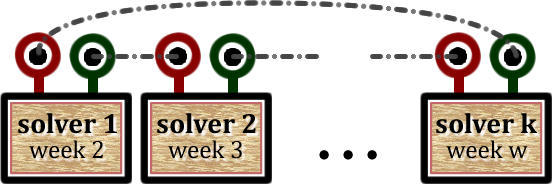
\includegraphics[width=0.45\linewidth]{golfers_ring.png}
	} %\hspace{0.1\linewidth}
	\subfloat[][]{%
		\label{subfig:golfers_bad_dic}
		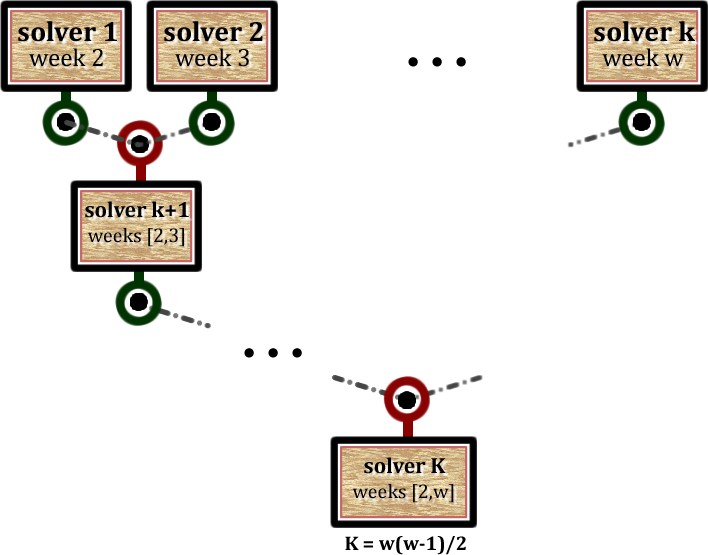
\includegraphics[width=0.45\linewidth]{golfers_dic.png}
	}
	\caption[]{Unsuccessful communication strategies to solve \SGP}
	\label{fig:golfers_bad}
\end{figure}

\separation

One last experiment using this benchmark was implementing a \commstr{} which applies a mechanism of cost descending acceleration, exchanging the current configuration between two solvers with different characteristics. Results show that this \commstr{} works pretty well for this problem.

For this strategy, new solvers were built reusing same \ms{} used for the \commstrs{} exposed before, and another different neighborhood \om{}: $V_{BP}(p)$, which given a configuration, returns the neighborhood $\mathcal{V}\left(s\right)$ by swapping the culprit player chosen for all $p$ randomly selected weeks with other players in the same week. This new solver was called \textit{companion solver}, and it descends quicker the cost of its current solution at the beginning because its neighborhood generates less values, but the convergence is slower and yet not sure. It was combined with the solver similar to the one used for the \commstrs{} exposed before. It was called \textit{standard solver}, and converges in a stable way to the solution. So, the companion solver uses the same neighborhood function that the standard solver, but parametrized in such a way that it builds neighbors only swapping players among two weeks.

The idea of the \commstr{} is to communicate a configuration from the companion solver to the standard solver, to be able to continue the search from a more promising place into de search space. After some iterations, is the standard solver who sends its configuration to the companion solver. The companion solver takes this received configuration and starts its search from it and finds quickly a much better configuration to send to the standard solver again. To force the companion solver to take the received configurations over its own, we use the \textit{not null} operator together with the \opch{} $C.M.$ (Algorithm~\ref{as:golfers_partial}). This process is repeated until a solution is found.

Figure~\ref{fig:solversgolfers} shows standard solver's run versus companion solver's run. In this chart we can see that, at the beginning of the run, found configurations by the companion solver have costs significantly lower than those found by the standard solver. \tet{At the 60-th millisecond} the standard solver current configuration has cost 123, and the companion solver's one, 76. So for example, the communication at this time, can accelerate the process significantly.

\begin{figure}
\centering
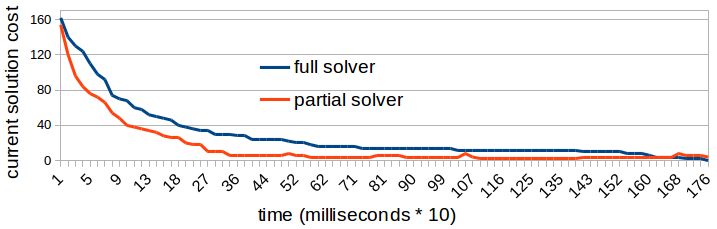
\includegraphics[width=0.9\columnwidth]{graph.png} 
\caption{Companion solver vs. standard solver (solving \sgp)}
\label{fig:solversgolfers}
\end{figure}

\begin{algorithm}
\dontprintsemicolon
\SetNoline
\SetKwProg{myproc}{\tet{\bf abstract solver}}{\tet{\bf begin}}{\tet{\bf end}}
\myproc{as\_standard \;
	\tet{\bf computation} : $I, V, S_1, S_2, A$\;
	\tet{\bf communication} : $C.M.$\;}{%
	$I \poslop{\mapsto}$
	\whileinline{$\left(\textbf{\Iter} < K_1\right)$}{
		$V \poslop{\mapsto} \left[S_1 \poslopcond{\Sci \% K_1} S_1\right] \poslop{\mapsto} \left[C.M. \poslop{m} \llparenthesis A \rrparenthesis^d\right]$		
	}
}
\tet{\bf solver} \solverposl{standard} \tet{\bf implements} as\_standard\;
\algoindent \tet{\bf computation} : $I_{BP}, V_{BAS}, S_{first}, S_{rand}, A_{AI}$ \;
\algoindent \tet{\bf communication} : $CM_{last}$ \;
\caption{Standard solver for \SGP}\label{as:golfers_full}
\end{algorithm}

\begin{algorithm}
\dontprintsemicolon
\SetNoline
\SetKwProg{myproc}{\tet{\bf abstract solver}}{\tet{\bf begin}}{\tet{\bf end}}
\myproc{as\_companion \;
	\tet{\bf computation} : $I, V, S_1, S_2, A$\;
	\tet{\bf communication} : $C.M.$\;}{
	$I \poslop{\mapsto}$
	\whileinline{$\left(\textbf{\Iter} < K_1\right)$}{
		$V \poslop{\mapsto} \left[S_1 \poslopcond{\Sci \% K_1} S_2\right] \poslop{\mapsto} \left[C.M. \poslop{\vee} \llparenthesis A \rrparenthesis^d\right]$		
	}
}
\tet{\bf solver} \solverposl{companion} \tet{\bf implements} as\_companion\;
\algoindent \tet{\bf computation} : $I_{BP}, V_{BP}(2), S_{first}, S_{rand}, A_{AI}$ \;
\algoindent \tet{\bf communication} : $CM_{last}$ \;
\caption{Companion solver for \SGP}\label{as:golfers_partial}
\end{algorithm}

We also design different \commstrs, combining connected and unconnected solvers in different percentages, and applying two different \commopers: \oneTone{} and \oneTn.

This strategy produces some gain in terms of runtime as we can see in Tables~\ref{tab:golfers_v2_1N} and \ref{tab:golfers_v2_11} with respect to Table~\ref{tab:golfersB001}. It produces also more robust results in terms of runtime. The spread of results in iterations show higher variances, because there are included also results of companion solvers, which performs many times more iterations that the standard solvers. The percentage of the receiver solvers that were able to find the solution before the others did, was significant (see Appendix~\ref{app:sgp}, Figures~\ref{barplot:5}, \ref{barplot:8} and \ref{barplot:9}). That shows that the communication played an important role during the search, despite inter--process communication's overheads (reception, information interpretation, making decisions, etc).

The code for the \commstr{} of 100\% of communicating solvers is presented in Algorithm~\ref{comm:golfers_v2_100} and for 50\% of communicating solvers in Algorithm~\ref{comm:golfers_v2_50}. 

\begin{algorithm}[H]
\dontprintsemicolon
\SetNoline
$\left[\eqsolverposl{companion}\cdot A\right] \onetoone \left[\eqsolverposl{standard}\cdot C.M.\right]20;$\;
$\left[\eqsolverposl{standard}\cdot A\right] \onetoone \left[\eqsolverposl{companion}\cdot C.M.\right]20;$
\caption{Companion communication strategy 100\% communication}\label{comm:golfers_v2_100}
\end{algorithm}

\begin{algorithm}[H]
\dontprintsemicolon
\SetNoline
$\left[\eqsolverposl{companion}\cdot A\right] \onetoone \left[\eqsolverposl{standard}\cdot C.M.\right]10;$\;
$\left[\eqsolverposl{standard}\cdot A\right] \onetoone \left[\eqsolverposl{companion}\cdot C.M.\right]10;$\;
$\left[\eqsolverposl{first}\right]20;$\;
\caption{Companion communication strategy 100\% communication}\label{comm:golfers_v2_50}
\end{algorithm}

\begin{table}
\captionsetup{belowskip=6pt,aboveskip=6pt}
\centering 
\renewcommand{\arraystretch}{1}
\resizebox{\columnwidth}{!}{%
\begin{tabular}{p{1.5cm}|R{0.8cm}R{1cm}R{0.6cm}R{1.1cm}|R{0.8cm}R{1cm}R{0.6cm}R{1.1cm}|R{0.8cm}R{1cm}R{0.6cm}R{1.1cm}}
	\hline 	
	\multirow{2}{*}{\centering {\bf Instance}} & \multicolumn{4}{c|}{Comm. \oneTn} & \multicolumn{4}{c}{(Comm. \oneTn)/2} & \multicolumn{4}{c}{(Comm. \oneTn)/4}\\
	\cline{2-13}
	& T & T(sd) & It. & It.(sd) & T & T(sd) & It. & It.(sd) & T & T(sd) & It. & It.(sd) \\
	\hline
	%\hline
	5--3--7 & 0.14 & 0.08 & 102 & 53 & 0.14 & 0.07 & 97 & 73 & 0.12 & 0.08 & 175 & 162 \\
	8--4--7 & 0.30 & 0.13 & 101 & 24 & 0.22 & 0.06 & 92 & 29 & 0.22 & 0.06 & 88 & 45 \\
	9--4--8 & 0.55 & 0.15 & 125 & 20 & 0.53 & 0.14 & 107 & 20 & 0.40 & 0.14 & 101 & 70 \\
	\hline
\end{tabular}
}
\caption{Companion \commstr{} with communication \oneTn}
\label{tab:golfers_v2_1N}
\end{table}

\begin{table}
\captionsetup{belowskip=6pt,aboveskip=6pt}
\centering 
\renewcommand{\arraystretch}{1}
\resizebox{\columnwidth}{!}{%
\begin{tabular}{p{1.5cm}|R{0.8cm}R{1cm}R{0.6cm}R{1.1cm}|R{0.8cm}R{1cm}R{0.6cm}R{1.1cm}|R{0.8cm}R{1cm}R{0.6cm}R{1.1cm}}
	\hline 	
	\multirow{2}{*}{\centering {\bf Instance}} & \multicolumn{4}{c|}{Comm. \oneTone{} (100\%)} & \multicolumn{4}{c|}{Comm. \oneTone{} (50\%)} & \multicolumn{4}{c}{Comm. \oneTone{} (25\%)}\\
	\cline{2-13}
	& T & T(sd) & It. & It.(sd) & T & T(sd) & It. & It.(sd) & T & T(sd) & It. & It.(sd) \\
	\hline
	%\hline
	5--3--7 & 0.10 & 0.05 & 98 & 75 & \good{0.08} & 0.04 & 139 & 122 & 0.11 & 0.05 & 190 & 142 \\
	8--4--7 & \good{0.14} & 0.05 & 100 & 64 & 0.22 & 0.06 & 119 & 74 & 0.21 & 0.5 & 101 & 64 \\
	9--4--8 & 0.37 & 0.14 & 86 & 65 & \good{0.36} & 0.12 & 144 & 92 & 0.45 & 0.11 & 150 & 96 \\
	\hline
\end{tabular}
}
\caption{companion \commstr{} with communication \oneTn}
\label{tab:golfers_v2_11}
\end{table}



%This confirms the intuition that parallel approach increases the probability of finding the solution within a more reasonable time (some tens of seconds), than with the sequential scheme \cite{Alon2011}. 
%The column labeled \textbf{\% success} in Table~\ref{tab:golfers_seq} indicates the percentage of solvers finding a solution before reaching a time--out (5 minutes). 
%presented in Table~\ref{tab:golfersB001}, column \textit{O.M. First Improvement} (without communication), and results with communication (Tables~\ref{tab:golfersB001comm100}, \ref{tab:golfersB001comm50} and \ref{tab:golfersB001comm25}). 

%\subsection{Analysis of results}
%
%
%
%
%\modified{Then we ran experiments to study \posl's behavior solving target problems in communicating scenarios. Some compositions of solvers set were taken into account:}
%\begin{inparaenum}[i.]
%	\item the structure of the communication (with/without communication or a mix), and
%	\item \modified{the used communication operator}.
%\end{inparaenum}

\section{Solving the \nqp}
\label{sec:nqueens}

In this section I present the performed study using \nqp{} (\NQP) as a benchmark. The \commstr{} analyzed here consists in exchanging cyclically the configuration between solvers using different neighborhood functions, in order to accelerate the process of generating very promising configurations. Final obtained results show that this \commstr{} works pretty well for some instances of this problem.

\subsection{Problem definition}

The \nqp{} (\NQP) asks how to place $N$ queens on a chess board so that none of them can hit any other in one move. This problem was introduced in 1848 by the chess player Max Bezzelas as the \textit{8-queen problem}, and years latter it was generalized as \textit{N-queen problem} by Franz Nauck. Since then many mathematicians, including Gauss, have worked on this problem. It finds a lot of applications, e.g., parallel memory storage schemes, traffic control, deadlock prevention, neural networks, constraint satisfaction problems, among others \cite{Bell2009}. Some studies suggest that the number of solution grows exponentially with the number of queens ($N$), but local search methods have been shown very good results for this problem \cite{Sosic1994}. For that reason we tested some communication strategies using \posl{}, to solve a problem relatively easy to solve using non communication strategies.

The cost function for this benchmark was implemented in C++ based on the current implementation of {\it Adaptive Search}\footnote{It is based on the code from Daniel D\'{i}az available at \href{https://sourceforge.net/projects/adaptivesearch/}{https://sourceforge.net/projects/adaptivesearch/}}.

\subsection{Experiments and results}

To handle this problem, some modules used for the \sgp{} have been reused: the selection \oms{} $S_{first}$ and $S_{best}$, and the acceptance \om{} $A_{AI}$. It was used a simple \as{} presented in Algorithm~\ref{as:nq}:

\begin{algorithm}[H]
\dontprintsemicolon
\SetNoline
\SetKwProg{myproc}{\tet{\bf abstract solver}}{\tet{\bf begin}}{\tet{\bf end}}
\myproc{as\_simple \tcp*{{\sc Itr} $\rightarrow$ number of iterations}
	\tet{\bf computation} : $I, V, S, A$\tcp*{{\sc Sci} $\rightarrow$ number of iterations with the same cost}}{
	$I \poslop{\mapsto}$
		\whileinline{$\left(\textbf{\Iter < } K_1\right)$}{$ V \poslop{\mapsto} S \poslop{\mapsto} A$}	
}
\tet{\bf solver} \solverposl{as} \tet{\bf implements} as\_simple\;
\algoindent \tet{\bf computation} : $I_{perm}, V_{AS}, S_{first}, A_{AI}$ \;
\tet{\bf solver} \solverposl{selective} \tet{\bf implements} as\_simple\;
\algoindent \tet{\bf computation} : $I_{perm}, V_{PAS}(p), S_{first}, A_{AI}$ \; 
%\tet{\bf connection}: $CM_{last}$\;
\caption{\As{} for \NQP}\label{as:nq}
\end{algorithm}

Solvers used for the experiments without communications, are presented in Algorithm~\ref{as:nq}, where the \as{} is instantiated in the solver \solverposl{as} with the neighborhood \om{} $V_{AS}$, which given a configuration, returns a neighborhood $V\left(s\right)$ swapping the variable which contributes the most to the cost, with all others. This solver was able to find solutions but taking too much time (a minute for 6000-queens, for example). For that reason it was implemented a neighborhood \om{} $S_{PAS}(p)$ which performs the same algorithm of $S_{AS}$, but instead of generating neighbors swapping the most costly variable with all others, it is swapped only with a percentage of rest of variables. Solver \solverposl{selective} instantiates the \as{} with this \om, showing much better results than \solverposl{as}.

Table~\ref{tab:nqueens_seqpar} presents results of sequential and parallel runs, using \solverposl{selective} with a tunned value of $p=2.5$. Results show that the improvement of the parallel scheme using \posl{} is not big. While the number of solutions of this problem is only known for the very small value of $N = 23$, studies suggest that the number of solutions grows exponentially with $N$. It implies that as the problem grows in order, it becomes easier to solve through local search methods. The behavior of \posl{} solving this problem matches  with this hypothesis: the search process solving larger instances is more stable and the convergence is direct. In a well spread search space with a lot of solutions, the parallelism using 40 cores do not provide a lot of improvement. In that sense, \modified{as a future work, experiments using \posl{} to solve \NQP{} in parallel with more cores are planned.}

\begin{table}[t]
\centering 
\renewcommand{\arraystretch}{1}
\resizebox{\columnwidth}{!}{%
\begin{tabular}{p{1.3cm}|R{1.3cm}R{1.3cm}R{1.3cm}R{1.3cm}|R{1.3cm}R{1.3cm}R{1.3cm}R{1.3cm}}
	\hline %\noalign{\smallskip}	
	\multirow{2}{*}{\footnotesize{\centering {\bf Instance}}} & \multicolumn{4}{c|}{\bf Sequential} & \multicolumn{4}{c}{\bf Parallel} \\
	\cline{2-9}
	& T & T(sd) & It. & It.(sd) & T & T(sd) & It. & It.(sd) \\	
	\hline
	250 & 0.29 & 0.072 & 8,898 & 2,158 & 0.19 & 0.003 & 4,139 & 913 \\
	500 & 0.35 & 0.087 & 4,203 & 998 & 0.24 & 0.036 & 2,675 & 366 \\
	1000 & 0.35 & 0.126 & 2,766 & 445 & 0.30 & 0.037 & 2,102 & 222 \\
	3000 & 1.50 & 0.138 & 2,191 & 77 & 1.33 & 0.055 & 2,168 & 71 \\
	6000 & 4.71 & 0.183 & 3,339 & 51 & 4.57 & 0.123 & 3,323 & 43 \\
	\hline
\end{tabular}
}
\caption{Results for \NQP{} (sequential and parallel without communication)}\label{tab:nqueens_seqpar}
\end{table}

\separation

In order to test the cooperative approach with this problem, a first and simple experiment was performed. Using the previous defined \as{}, communicating solvers were built, to create a simple \commstr{} in which the shared information is the current configuration, and it is communicated in one sense (from sender solvers to receivers). Algorithms~\ref{as:nq_sender}~and~\ref{as:nq_receiver} show that the communication is performed while applying the acceptance criterion. We design different communication strategies: 
\begin{itemize}
\item a set of sender solvers sending information to receiver solvers, using operator \oneTone{} (see see Algorithm~\ref{comm:nqueens_simple_11}) and operator \oneTn{} (see Algorithm~\ref{comm:nqueens_simple_1nk} with $K=1$)
\item some sets of sender solvers sending information to receiver solvers, using operator \oneTn{} (see see Algorithm~\ref{comm:nqueens_simple_1nk}), with $K\in\left\{2, 4\right\}$
\end{itemize}

\begin{algorithm}[H]
\dontprintsemicolon
\SetNoline
\SetKwProg{myproc}{\tet{\bf abstract solver}}{\tet{\bf begin}}{\tet{\bf end}}
\myproc{as\_sender \tcp*{{\sc Itr} $\rightarrow$ number of iterations}
	\tet{\bf computation} : $I, V, S, A$\tcp*{{\sc Sci} $\rightarrow$ number of iterations with the same cost}}{
	$I \poslop{\mapsto}$
		\whileinline{$\left(\textbf{\Iter < } K_1\right)$}{$ V \poslop{\mapsto} S \poslop{\mapsto} \llparenthesis A \rrparenthesis^d$}	
}
\tet{\bf solver} \solverposl{sender} \tet{\bf implements} as\_sender\;
\algoindent \tet{\bf computation} : $I_{perm}, V_{PAS}(p), S_{first}, A_{AI}$ \;
\caption{Sender solver for \NQP{} (simple \commstr)}\label{as:nq_sender}
\end{algorithm}

\begin{algorithm}[H]
\dontprintsemicolon
\SetNoline
\SetKwProg{myproc}{\tet{\bf abstract solver}}{\tet{\bf begin}}{\tet{\bf end}}
\myproc{as\_receiver \tcp*{{\sc Itr} $\rightarrow$ number of iterations}
	\tet{\bf computation} : $I, V, S, A$\tcp*{{\sc Sci} $\rightarrow$ number of iterations with the same cost}
	\tet{\bf communication} : $C.M.$\;}{%
	$I \poslop{\mapsto}$
		\whileinline{$\left(\textbf{\Iter < } K_1\right)$}{$ V \poslop{\mapsto} S \poslop{\mapsto} \left[A \poslopcond{\Iter \% K_2} \left[A \poslop{m} C.M.\right]\right]$}
}
\tet{\bf solver} \solverposl{receiver} \tet{\bf implements} as\_receiver\;
\algoindent \tet{\bf computation} : $I_{perm}, V_{PAS}(p), S_{first}, A_{AI}$ \;
\algoindent \tet{\bf communication}: $CM_{last}$\;
\caption{Receiver solver for \NQP{} (simple \commstr)}\label{as:nq_receiver}
\end{algorithm}

\begin{algorithm}[H]
\dontprintsemicolon
\SetNoline
$\left[\eqsolverposl{sender}\posldot A\right] \onetoone \left[\eqsolverposl{receiver}\posldot C.M.\right]20;$
\caption{Simple \commstr{} \oneTone{} for \NQP}\label{comm:nqueens_simple_11}
\end{algorithm}

\begin{algorithm}[H]
\dontprintsemicolon
\SetNoline
$\left[\eqsolverposl{sender}\posldot A(\tfrac{20}{K})\right] \oneton \left[\eqsolverposl{receiver}\posldot C.M.(\tfrac{20}{K})\right]K;$
\caption{Simple \commstr{} \oneTn{} for \NQP}\label{comm:nqueens_simple_1nk}
\end{algorithm}

Tables~\ref{tab:nqueens_simplecomm11} and ~\ref{tab:nqueens_simplecomm1n} show how the communication improve the non communicating results in terms of runtime and iterations, but this improvement is not significant. In contrast to \SGP, \posl{} does not get trapped so often into local minima during the resolution of \NQP{}. For that reason, the shared information, once received and accepted by the receivers solvers, does not improves largely the current cost.

\begin{table}[t]
\centering 
\renewcommand{\arraystretch}{1}
\newcommand{\cwnq}{1.1cm}
\begin{tabular}{p{1.3cm}|R{\cwnq}R{\cwnq}R{\cwnq}R{\cwnq}}
	\hline 
	\multirow{2}{*}{\footnotesize{\centering {\bf Instance}}} & \multicolumn{4}{c}{\bf Communication 1-1} \\
	\cline{2-5}
	& T & T(sd) & It. & It.(sd) \\	
	\hline
	250 & 0.18 & 0.040 & 3,433 & 697 \\ 
	500 & 0.25 & 0.047 & 2,216 & 427 \\
	1000 & 0.26 & 0.056 & 1,735 & 424\\
	3000 & 1.21 & 0.088 & 1,873 & 227\\
	6000 & 4.38 & 0.111 & 3,178 & 121\\	
	\hline
\end{tabular}
\caption{Simple \commstr{} \oneTone{} for \NQP}\label{tab:nqueens_simplecomm11}
\end{table}

\begin{table}[h]
\centering 
\renewcommand{\arraystretch}{1}
\newcommand{\cwnq}{1.1cm}
\resizebox{\columnwidth}{!}{%
\begin{tabular}{p{1.3cm}|R{\cwnq}R{\cwnq}R{\cwnq}R{\cwnq}|R{\cwnq}R{\cwnq}R{\cwnq}R{\cwnq}|R{\cwnq}R{\cwnq}R{\cwnq}R{\cwnq}}
	\hline %\noalign{\smallskip}	
	\multirow{2}{*}{\footnotesize{\centering {\bf Instance}}} & \multicolumn{4}{c|}{\bf Communication 1-n} & \multicolumn{4}{c|}{\bf Communication (1-n)$\times$2} &  \multicolumn{4}{c}{\bf Communication (1-n)$\times$4}\\
	\cline{2-13}
	& T & T(sd) & It. & It.(sd) & T & T(sd) & It. & It.(sd) & T & T(sd) & It. & It.(sd) \\	
	\hline
	250 & 0.16 & 0.032 & 2,621 & 894 & 0.15 & 0.036 & 2,459 & 892 & 0.15 & 0.036 & 2,494 & 547\\
	500 & 0.20 & 0.040 & 1,592 & 428 & 0.19 & 0.053 & 1,521 & 539 & 0.18 & 0.057 & 1,719 & 593\\
	1000 & 0.26 & 0.055 & 1,329 & 286 & 0.25 & 0.046 & 1,435 & 369 & 0.23 & 0. 056 & 1,400 & 426\\
	3000 & 1.26 & 0.078 & 1,657 & 212 & 1.22 & 0.101 & 1,598 & 249 & 1.20 & 0.078 & 1,704 & 252\\
	6000 & 4.40 & 0.118 & 2,771 & 197 & 4.35 & 0.127 & 2,840 & 148 & 4.33 & 0.120 & 2,975 & 188\\	
	\hline
\end{tabular}
}
\caption{Simple \commstr{} \oneTn{} for \NQP}\label{tab:nqueens_simplecomm1n}
\end{table}

\separation

In the following experiment, with the goal of improving results, another \commstr{} was implemented, very similar to the one applied to \SGP{}, but in this case, with solvers using the same neighborhood function $V_{PAS}(p)$ but with different values of $p$ and different selection functions. In this \commstr{} a cyclic exchange of the current configuration is performed between to different solvers. One solver \textit{companion} using the neighborhood \om{} $V_{PAS}(p)$ with a smaller value of $p$ and using the selection \om{} $S_{best}$, meaning that it is able to find promising configuration faster, but its convergence is slower. 
The other solver is very similar to the one used for non communicating experiments, but in this \commstr{} solvers are both senders and receivers (see Algorithm~\ref{as:nq_cyc}). Before designing \commstrs{} (Algorithms~\ref{comm:nqueens_cyc_11}, and ~\ref{comm:nqueens_cyc_1n}), many experiments were launched to select: \begin{inparaenum} \item The percentage of variables that the companion solver swaps with the culprit one, when executing the neighborhood \om{} ($p$). This value was decided to be $1$. \item The number of companion solvers to connect with the standard one, for the \commstr{} using operator \oneTn. This vale was decide to be $2$, as we can see in Algorithm~\ref{comm:nqueens_cyc_1n}. \end{inparaenum} 

\begin{algorithm}[H]
\dontprintsemicolon
\SetNoline
\SetKwProg{myproc}{\tet{\bf abstract solver}}{\tet{\bf begin}}{\tet{\bf end}}
\myproc{as\_cyc \tcp*{{\sc Itr} $\rightarrow$ number of iterations}
	\tet{\bf computation} : $I, V, S_1, S_2, A$\tcp*{{\sc Sci} $\rightarrow$ number of iterations with the same cost}
	\tet{\bf communication} : $C.M.$\;}{%
	$I \poslop{\mapsto}$
		\whileinline{$\left(\textbf{\Iter < } K_1\right)$}{$ V \poslop{\mapsto} S \poslop{\mapsto} \left[A \poslopcond{\Iter \% K_2} \left[\llparenthesis A \rrparenthesis^d \poslop{m} C.M.\right]\right]$}
}
\tet{\bf solver} \solverposl{standard} \tet{\bf implements} as\_cyc\;
\algoindent \tet{\bf computation} : $I_{perm}, V_{PAS}(2.5), S_{first}, A_{AI}$ \;
\algoindent \tet{\bf communication}: $CM_{last}$\;
\tet{\bf solver} \solverposl{companion} \tet{\bf implements} as\_cyc\;
\algoindent \tet{\bf computation} : $I_{perm}, V_{PAS}(1), S_{best}, A_{AI}$ \;
\algoindent \tet{\bf communication}: $CM_{last}$\;
\caption{Solvers for cyclic \commstr{} to solve \NQP{}}\label{as:nq_cyc}
\end{algorithm}

\begin{algorithm}[H]
\dontprintsemicolon
\SetNoline
$\left[\eqsolverposl{companion}\posldot A\right] \onetoone \left[\eqsolverposl{standard}\posldot C.M.\right]20;$\;
$\left[\eqsolverposl{standard}\posldot A\right] \onetoone \left[\eqsolverposl{companion}\posldot C.M.\right]20;$
\caption{Cyclic \commstr{} \oneTone{} for \NQP}\label{comm:nqueens_cyc_11}
\end{algorithm}

\begin{algorithm}[h]
\dontprintsemicolon
\SetNoline
$\left[\eqsolverposl{companion}\posldot A(2)\right] \oneton \left[\eqsolverposl{standard}\posldot C.M.\right]13;$\;
$\left[\eqsolverposl{standard}\posldot A\right] \oneton \left[\eqsolverposl{companion}\posldot C.M.(2)\right]13;$
\caption{Cyclic \commstr{} \oneTn{} for \NQP}\label{comm:nqueens_cyc_1n}
\end{algorithm}

\begin{table}[h]
\centering 
\renewcommand{\arraystretch}{1}
\newcommand{\cwnq}{1.1cm}
\resizebox{\columnwidth}{!}{%
\begin{tabular}{p{1.3cm}|R{\cwnq}R{\cwnq}R{\cwnq}R{\cwnq}|R{\cwnq}R{\cwnq}R{\cwnq}R{\cwnq}|R{\cwnq}}
	\hline %\noalign{\smallskip}	
	\multirow{2}{*}{\footnotesize{\centering {\bf Instance}}} & \multicolumn{4}{c|}{\bf Communication 1-1} & \multicolumn{4}{c|}{\bf Communication 1-n}&\multirow{2}{*}{\centering {\bf I.R.}}\\
	\cline{2-9}
	& T & T(sd) & It. & It.(sd) & T & T(sd) & It. & It.(sd)&\\	
	\hline
	250 & \good{0.09} & 0.021 & 1,169 & 254 & 0.10 & 0.021 & 1,224 & 254 & 2.00\\ 
	500 & \good{0.14} & 0.027 & 864 & 121 & 0.15 & 0.030 & 977 & 220 & 1.65\\
	1000 & 0.22 & 0.041 & 889 & 247 & \good{0.21} & 0.056 & 807 & 196& 1.39\\
	3000 & 1.25 & 0.090 & 1,602 & 90 & \good{1.02} & 0.145 & 1,613 & 206 & 1.17\\
	6000 & 4.83 & 0.121 & 2,938 & 746 & \good{4.24} & 0.746 & 2,537 & 779 & 1.01\\	
	\hline
\end{tabular}
}
\caption{Cyclic \commstr{} for \NQP}\label{tab:nqueens_cyc}
\end{table}

With this experiment, it was possible to find a \commstr{} which improves runtimes significantly, but only for small instances of the problem, where the number of solutions, with respect to the order $N$, is lower. This result confirms experimentally the hypothesis already introduced, which propose that as the size of the problem grows, (and with it, the number ef solutions inside the search space with respect to $N$) lower is the gain using communication during the search process. Table~\ref{tab:nqueens_cyc} shows how the \textit{improvement ratio} (column \textbf{I.R.}) decreases with the instance order $N$. This ratio was computed using the following equation:

\[
\frac{\mbox{runtime without communication}}{\frac{\left(\mbox{runtime using communication 1-1} + \mbox{runtime using communication 1-n}\right)}{2}}
\] 

%\pgfplotsset{
%	myStyle/.style={grid=major,font=\Large}, ylabel= Communication rate,
%	xlabel=Number of cores,
%	legend style={at={(0.7,0.9)},
%	anchor=north}
%}

%\begin{figure}
%\centering
%\begin{tikzpicture} [scale=0.7]
%\begin{groupplot}[
%group style={
%	group name=my plots,
%	group size=1 by 5,
%	xlabels at=edge bottom,
%	xticklabels at=edge bottom,		
%	ylabels at=edge left,
%	yticklabels at=edge left,
%	vertical sep=0pt
%},
%legend style={at={(0.32,0.40)},anchor=north, legend columns=2},
%footnotesize,
%width=14cm,
%height=4.5cm,
%xlabel=\% of communicating solvers,
%ylabel= \empty,
%xmin=-5,
%xmax=105,
%ymin=0,	
%ymax=30,
%ytick={0,10,...,20},
%xtick={0,25,50,100},
%tickpos=left,
%ytick align=outside,
%xtick align=outside]
%
%\nextgroupplot %2000
%[ymin=5.6, ymax=6.2, ytick={5.7,5.8,5.9,6.0,6.1,6.2}, cycle list ={{red, mark options={fill=red,scale=0.8},mark=*}, {blue, mark options={fill=blue,scale=0.8},mark=*}, {green, mark options={fill=green,scale=0.8},mark=*}, {orange, mark options={fill=orange,scale=0.8},mark=x}}]
%\addlegendentry{1 to 1}
%\addplot coordinates{(0,6.15) (25,6.05) (50,6.01) (100,5.92)};
%\addlegendentry{1 to N}
%\addplot coordinates{(0,6.15) (25,6.07) (50,5.98) (100,6.01)};
%
%\nextgroupplot %3000
%[ymin=13.5, ymax=14.1, ytick={13.6,13.7,13.8,13.9,14.0,14.1}, cycle list ={{red, mark options={fill=red,scale=0.8},mark=*}, {blue, mark options={fill=blue,scale=0.8},mark=*}, {green, mark options={fill=green,scale=0.8},mark=*}, {orange, mark options={fill=orange,scale=0.8},mark=x}}]
%\addplot coordinates{(0,14.06) (25,13.89) (50,13.91) (100,13.67)};
%\addplot coordinates{(0,14.06) (25,13.97) (50,13.96) (100,13.79)};
%
%\nextgroupplot %4000
%[ymin=24.9, ymax=25.5, ytick={25.0,25.1,25.2,25.3,25.4,25.5}, cycle list ={{red, mark options={fill=red,scale=0.8},mark=*}, {blue, mark options={fill=blue,scale=0.8},mark=*}, {green, mark options={fill=green,scale=0.8},mark=*}, {orange, mark options={fill=orange,scale=0.8},mark=x}}, ylabel= runtime (secs)]
%\addplot coordinates{(0,25.46) (25,25.25) (50,25.14) (100,25.11)};
%\addplot coordinates{(0,25.46) (25,25.30) (50,25.29) (100,25.17)};
%
%\nextgroupplot %5000
%[ymin=39.5, ymax=40.7, ytick={39.6,39.8,40.0,40.2,40.4,40.6}, cycle list ={{red, mark options={fill=red,scale=0.8},mark=*}, {blue, mark options={fill=blue,scale=0.8},mark=*}, {green, mark options={fill=green,scale=0.8},mark=*}, {orange, mark options={fill=orange,scale=0.8},mark=x}}]
%\addplot coordinates{(0,40.57) (25,40.38) (50,40.33) (100,39.62)};
%\addplot coordinates{(0,40.57) (25,40.45) (50,40.37) (100,39.88)};
%
%\nextgroupplot %6000
%[ymin=58.8, ymax=60.4, ytick={58.8,59.1,59.4,59.7,60.0,60.3}, cycle list ={{red, mark options={fill=red,scale=0.8},mark=*}, {blue, mark options={fill=blue,scale=0.8},mark=*}, {green, mark options={fill=green,scale=0.8},mark=*}, {orange, mark options={fill=orange,scale=0.8},mark=x}}]
%\addplot coordinates{(0,60.10) (25,59.28) (50,58.97) (100,58.97)};
%\addplot coordinates{(0,60.10) (25,59.77) (50,59.53) (100,59.16)};
%		
%\end{groupplot}
%\end{tikzpicture}
%\caption[]{Runtime means of instances \\2000-, 3000-, 4000-, 5000- and 6000-queens}
%\label{fig:results_nq}
%\end{figure}


%\modified{Results in Table~\ref{tab:nqueens_dic}} show that this strategy is effective to solve the \nqp{} improving the runtimes already obtained in the previews experiment. In the resolution of this problem, the improvement rate of the current configuration cost is very slow (yet stable). The \textit{partial} solvers work only on a section of the configuration, and for that reason, they are able to obtain configuration with costs considerably lower than the obtained by the {\it full} solver more quickly. This characteristic is taken into account: \textit{partial} solvers send their obtained configurations to the \textit{full} solvers. By doing this, the improvement rate of the current configuration can be accelerated at the beginning of the search.

\section{Solving the \carrp}
\label{sec:costas}

\new{In this section I present a performed study using \carrp{} (\CARRP) as a benchmark, by testing a simple communication strategy, in which the information to communicate between solvers is the current configuration received at different times of the algorithm. Results show that for this problem, this strategy improve the parallel non cooperative approach.}

\subsection{Problem definition}

The \carrp{} (\CARRP) consists in finding a \textit{costas array}, which is an $n\times n$ grid containing $n$ marks such that there is exactly one mark per row and per column and the $n(n-1)/2$ vectors joining each couple of marks are all different. This is a very complex problem that finds useful application in some fields like sonar and radar engineering.

\new{\CARRP{} has been studied for several years, and yet many questions remain open, like for example the existence of solutions for all $n$, the existence of other construction algorithms, among others \cite{Rickard}. It also presents an interesting characteristic: although the search space grows factorially, from order 17 the number of solutions drastically decreases~\cite{Drakakis2006}. For example, using the Golomb \cite{Golomb1984a} and Welch \cite{Golomb1984} constructions, \etal{Drakakis} present in~\cite{Drakakis2011} all Costas arrays for $n = 29$, and they show that among the $29!$ permutations, there are only 164 Costas arrays. Nowadays, after many decades of research, the problem of knowing whether it  exists any Costas array for $n = 32$ remains open \cite{Caniou14}.}

\new{For modeling this benchmark as an unconstrained optimization problem, the proposed model has $N$ variables: $\left\{v_1, v_2, \dots, v_n\right\}$, and their domains are the same: $D_{v_i}=\left\{1, \dots, n\right\}$.}

\new{The cost function for \CARRP{} was implemented in C++ based on the current implementation of Adaptive Search\footnote{It is based on the code from Daniel D\'{i}az available at \href{https://sourceforge.net/projects/adaptivesearch/}{https://sourceforge.net/projects/adaptivesearch/}}. It assumes that a configuration $s$ is an integer permutation of the set $\left\{1...n\right\}$, i.e. $s_i = j$ (the $i^{th}$ variable has the value $j$) means that there is a mark placed in column $i$ and row $j$. In that sense, the cost function does not verifies whether values in $s$ are all different.}

\new{The cost is computed by building the triangular matrix of all \textit{diferences} between marks. A difference between two marks $m_i$ and $m_j$ is defined as the vertical shift of $m_j$ with respect to $m_i$. For example, if the mark $m_i$ (mark placed on column $i$) is placed on the row 4, and the mark $m_j$ (mark placed on column $j$) is placed on the row 3, the difference between them is $4-3=1$. The following example describe a differences triangle for a $5\times 5$ matrix:}

\poslexample{Figure\ref{fig:ex_costas} shows a $5\times 5$ matrix with marks. The corresponding configuration for the \carrp{} is the following:
$$s=\left\{3, 2, 4, 5, 1\right\}$$
Its differences triangle is defined as follows:
\begin{equation*}
\begin{tabular}{cll}
3\hspace{10pt}2\hspace{10pt}4\hspace{10pt}5\hspace{10pt}1 & $\rightarrow$ & $d_0=s$\\
1\hspace{7pt}-2\hspace{7pt}-1\hspace{10pt}4 & $\rightarrow$ & $d_1$ \\
-1\hspace{7pt}-3\hspace{10pt}3 & $\rightarrow$ & $d_2$ \\
-2\hspace{10pt}1 & $\rightarrow$ & $d_3$ \\
2 & $\rightarrow$ & $d_4$
\end{tabular}
\end{equation*}
In this triangular matrix, row $i$ is denoted by $d_i$, which represent the difference between elements of $s$ located between each other at a distance $i$. For example, $d_3$ are the differences of values from $s$ located between each other at a distance $3$, so 
\begin{align*}
d_3 &= \left\{s_0-s_3, s_1-s_4\right\}\\
d_3 &= \left\{3-5, 2-1\right\}\\
d_3 &= \left\{-2, 1\right\}
\end{align*}

}

\begin{figure}[h]
\centering
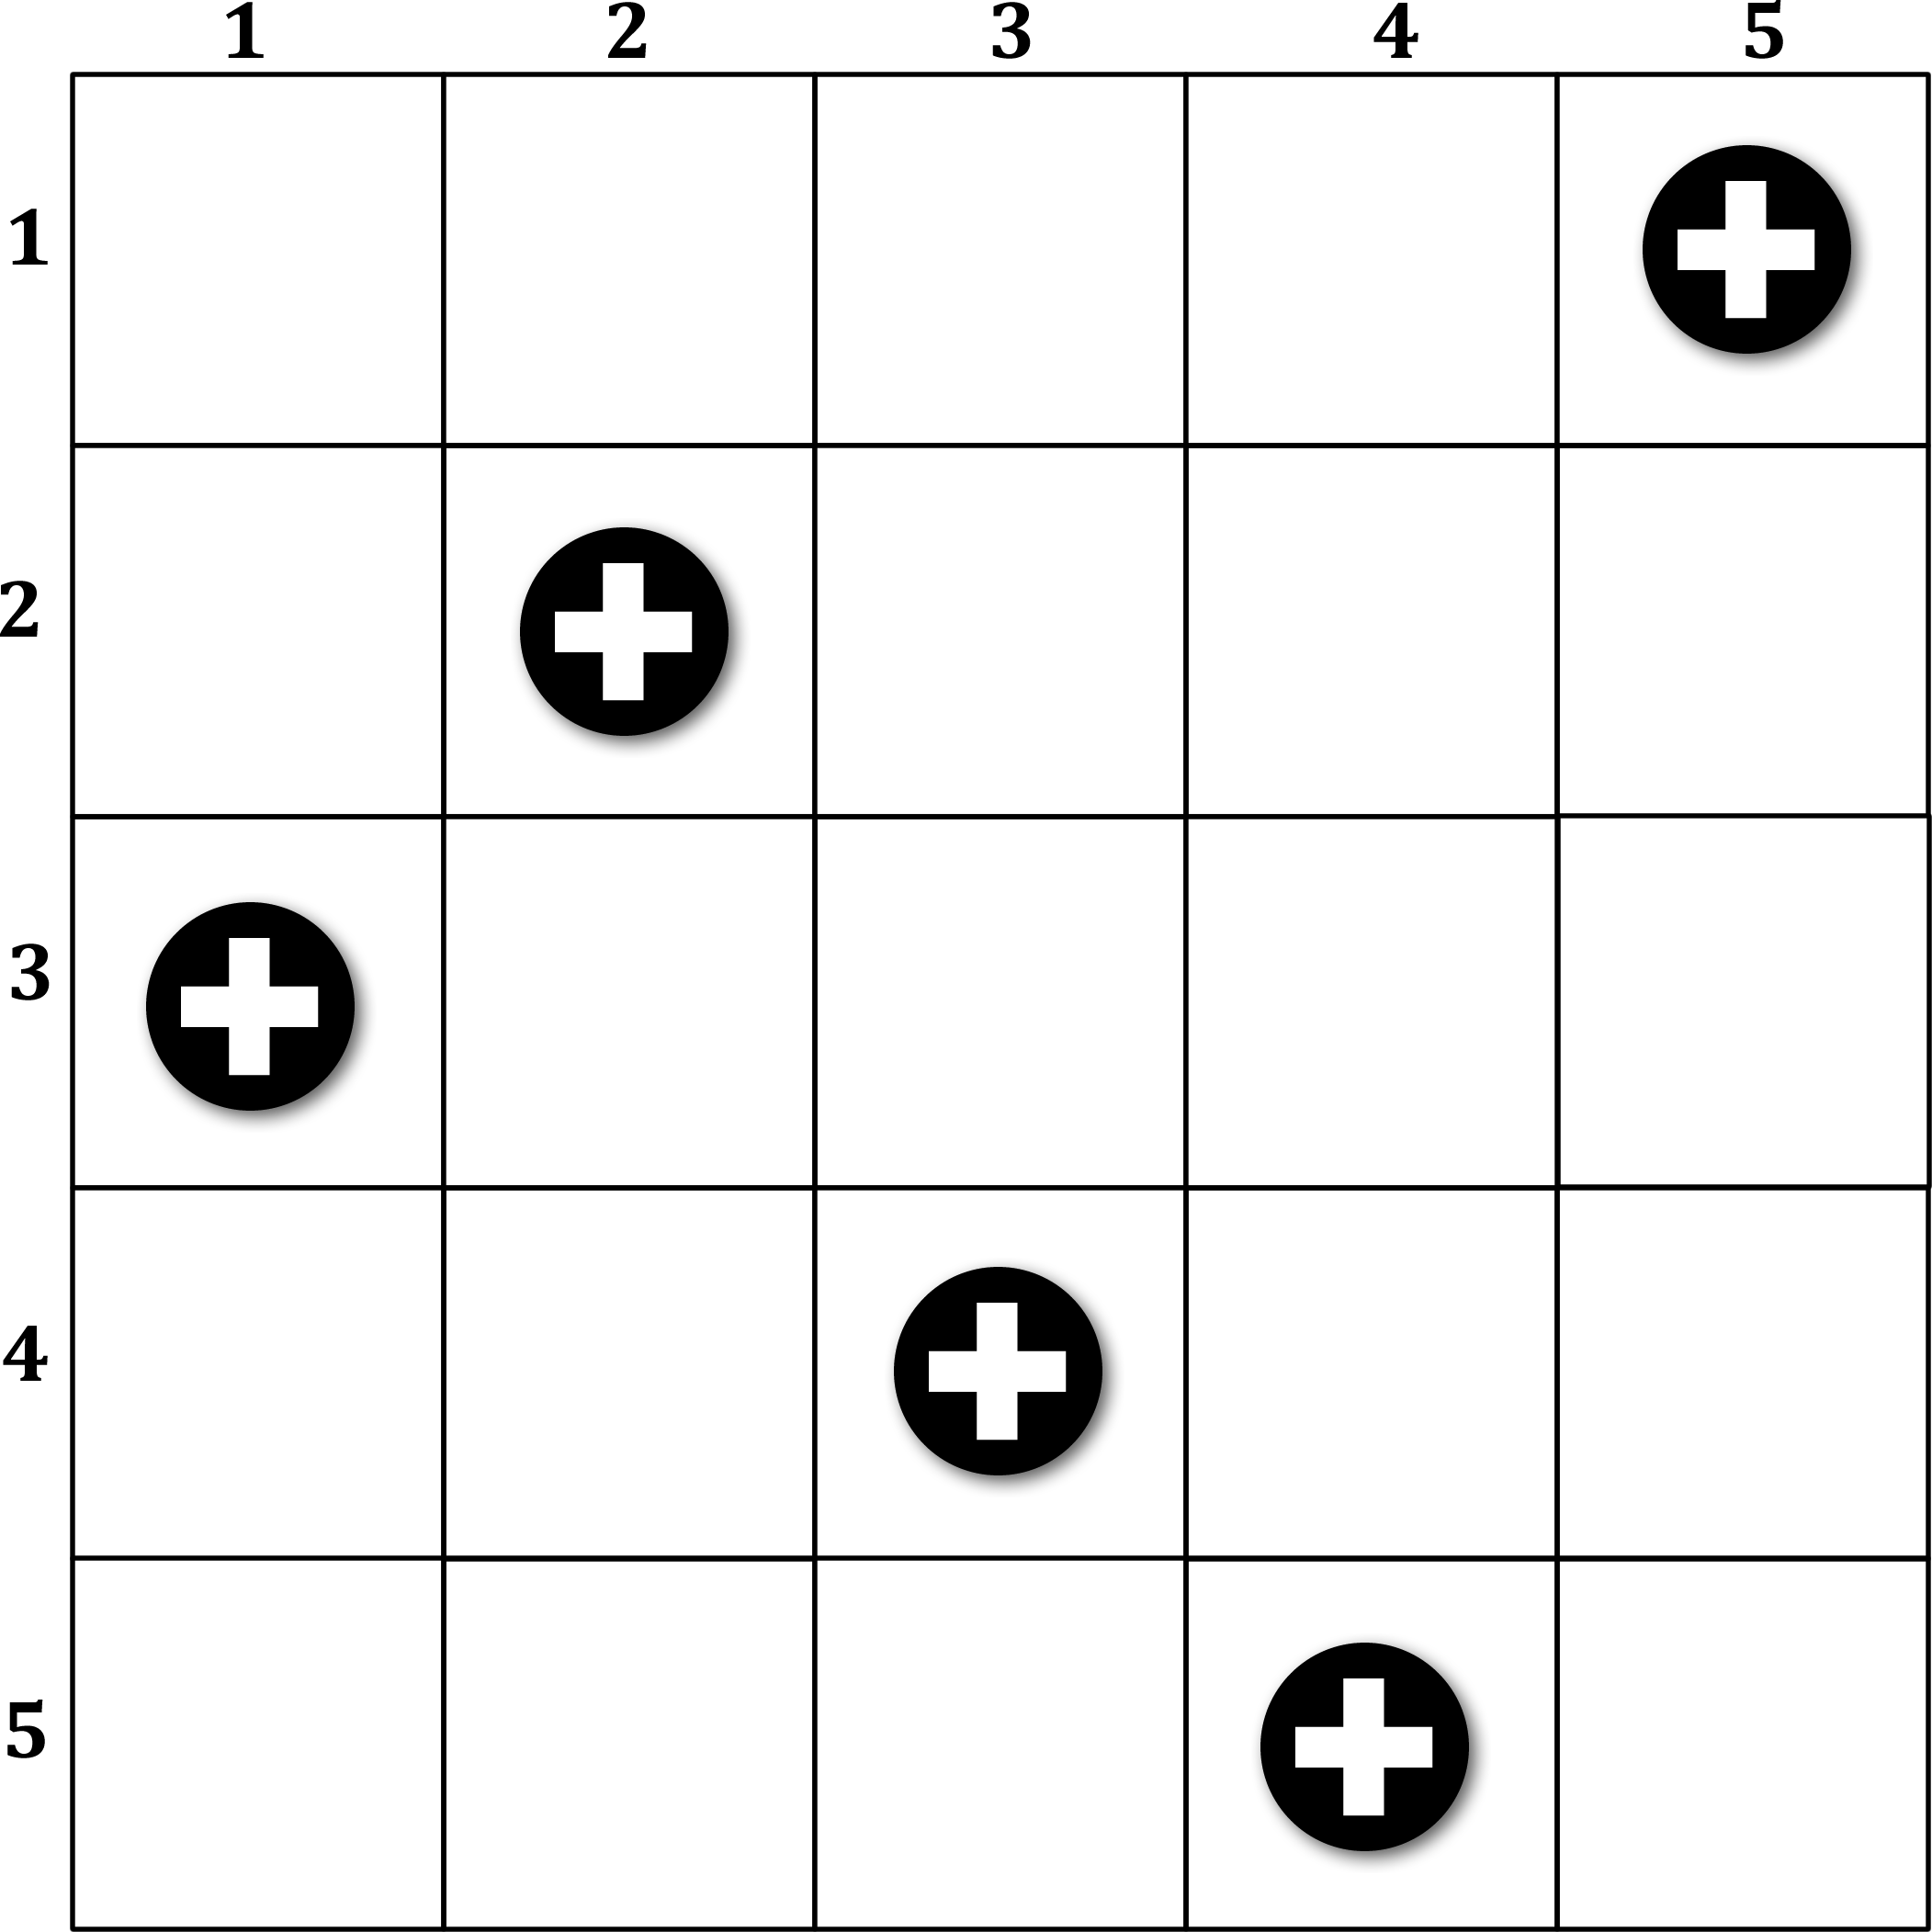
\includegraphics[width=0.35\linewidth]{costas.png}
\caption[]{Example of marks for \CARRP}
\label{fig:ex_costas}
\end{figure}

\new{The cost of the configuration $s$ is then the number of equal elements on each row $d_i$ of its corresponding differences triangle. It can be easily proved that this differences triangle is only necessary to be verified until the row $d_B$, with $B=\floor*{(n-1)/2}$.}

\subsection{Experiments design and results}

To handle this problem, I have reused all modules used for solving the \nqp. First attempts to solve this problems were using the same strategies (\ass) used to solve the \sgp{} and \nqp, without success: \posl{} was not able to solve instances larger than $n = 8$ in a reasonable amount of time (seconds). After many unsuccessful attempts to find the right parameters of \textit{maximum number of restarts}, \textit{maximum number of iterations}, and \textit{maximum number of iterations with the same cost}, I decided to implement the mechanism used by Daniel D\'iaz in the current implementation of {\it Adaptive Search} to escape from local minima: I have added a {\it Reset} \om{} $R_{AS}$ based on the abstract \om{} $R$. The other \oms{} were the same used for solving the \nqp.

Given a configuration $s$, the basic principle of the reset is build another following four steps:
\begin{enumerate}
\item A configuration is obtained by performing left/right shifts to all sub-vectors of $s$ starting or ending by the variable which contributes the most to the cost, and selecting the configuration with the lowest cost.
\item A configurations is obtained by adding a constant (circularly) to each element in the configuration $s$.
\item A configuration is obtained by shifting left from the beginning of $s$ to some culprit variable (i.e. a variable contributing to the cost).
\item Then, one of these 3 generated configuration has the same probability of being selected, to be the result of the reset algorithm. In that sense, some different resets can be performed for the same configuration.
\end{enumerate}


The basic solver used to solve this problem is presented in Algorithm~\ref{as:costas}, and it was taken as a base to build all the different communication strategies. Basically, it is a classical local search iteration, where instead of performing restarts, it performs resets. After a deep analysis of this implementation and results of some runs, I decided to use $K_1 = 2,000,000$ (maximum number of iterations) big enough to solve the chosen instance $n = 19$; and $K_2 = 3$ (the number of iteration before performing the next \textit{reset}).

\begin{algorithm}[H]
\dontprintsemicolon
\SetNoline
\SetKwProg{myproc}{\tet{\bf abstract solver}}{\tet{\bf begin}}{\tet{\bf end}}
\myproc{as\_hard \tcp*{{\sc Itr} $\rightarrow$ number of iterations}
	\tet{\bf computation} : $I, R, V, S, A$\;}{ %\tcp*{{\sc Sci} $\rightarrow$ number of iterations with the same cost}}{%
	$I \poslop{\mapsto}$
	\whileinline{$\left(\textbf{\Iter < } K_1\right)$}{
		$R \poslop{\mapsto}$ % \left[\circlearrowleft (\text{\Iter}\% K_2) \left\{ M_V \longmapsto M_{\hat{S}} \longmapsto M_D\right\}\right]$\;
		\whileinline{$\left(\textbf{\Iter \% } K_2\right)$}{$\left[V \poslop{\mapsto} S \poslop{\mapsto} A\right]$}
	}
}
\tet{\bf solver} \solverposl{single} \tet{\bf implements} as\_hard\;
\algoindent \tet{\bf computation} : $I_{perm},  R_{AS}, V_{AS}, S_{first}, A_{AI}$ \;
%\tet{\bf connection}: $CM_{last}$\;
\caption{Reset-based \as{} for \CARRP}\label{as:costas}
\end{algorithm}

Table~\ref{tab:costas19} shows results of launching \sosets{} to solve each instance of \carrp{} 19 sequentially and in parallel without communication. Runtimes and iteration means showed in this confirm once again the success of the parallel approach. 

\begin{table}[h]
\captionsetup{belowskip=6pt,aboveskip=6pt}
\centering
\renewcommand{\arraystretch}{1}
\begin{tabular}{p{3.5cm}|R{1.5cm}R{1cm}R{1.7cm}R{1.7cm}R{2cm}}
	\hline
	{\bf STRATEGY} & T & T(ds) & It. & It.(sd) & \% success\\
	\hline
	%\hline
	Sequential (1 core) & 132.73 & 80.32 & 2,332,088 & 1,424,757 & 40.00\\
	Parallel (40 cores) & 25.51 & 15.75 & 231,262 & 143,789 & 100.00\\
	\hline
\end{tabular}
\caption{\carr{} 19: no communication}
\label{tab:costas19}
\end{table}

\separation

In order to improve results, a simple communication strategy was applied: communicating the current configuration to other solvers. To do so, we insert a \textit{sending output} operator to the \as{} in Algorithm~\ref{as:costas}. This results in the sender solver presented in Algorithm~\ref{as:costas_sender}. %\tet{et le receiver??? Flo: c'est l'algo 4}

\begin{algorithm}[h]
\dontprintsemicolon
\SetNoline
\SetKwProg{myproc}{\tet{\bf abstract solver}}{\tet{\bf begin}}{\tet{\bf end}}
\myproc{as\_hard\_sender \; %\hspace{3pt}
	\tet{\bf computation} : $I, R, V, S, A$\;}{
	$I \poslop{\mapsto}$
	\whileinline{$\left(\textbf{\Iter} < K_1\right)$}{
		$T \poslop{\mapsto}$
		\whileinline{$\left(\textbf{\Iter \% } K_2\right)$}{$\left[V \poslop{\mapsto} S \poslop{\mapsto} \llparenthesis A \rrparenthesis^d\right]$}
	}
}
\tet{\bf solver} \solverposl{sender} \tet{\bf implements} as\_hard\_sender\;
\algoindent \tet{\bf computation} : $I_{perm}, R_{AS}, V_{AS}, S_{first}, A_{AI}$ \;
%\tet{\bf connection}: $CM_{last}$\;
\caption{Sender solver for \CARRP}\label{as:costas_sender}
\end{algorithm}

Studying some runs of \posl{} solving \CARRP{}, it was observed that \new{during the search process, the cost of the current configuration of all solvers describes an oscillatory descent due to the repeated resets ($K_2 = 3$ in Algorithm~\ref{as:costas}). It means that the cost of the current configuration decreases during $K_2$ iterations and then the current configuration is created by performing a reset which generates generally a more costly configuration. However, in every performed experiment (more than 20 runs with 20 solvers in parallel without communication), the current configuration's cost of the winner solver (first solver finding a solution) described an oscillatory descent also, but not so pronounced (i.e. the difference between the cost of the last current configuration before performing the reset and the cost of the configuration after the reset is not high).} For that reason, it was decided to apply a simple \commstr{} that shares the current configuration while applying the acceptance criterion. To do so, a \opch{} using a \textit{minimum} operator $\poslop{m}$ together with the abstract \om{} $A$ was inserted, as shown in Algorithm~\ref{as:costas_receiver_a}.

One of the main purpose of this study is to explore different communication strategies. We have then implemented and tested different variations of the strategy exposed above by combining two communication operators (\oneTone{} and \oneTn) and different percentages of communicating solvers.
For this problem, it was study also the behavior of the communication performed at two different moments: while applying the acceptance criteria (Algorithm~\ref{as:costas_receiver_a}), and while performing a {\it reset} (Algorithm~\ref{as:costas_receiver_b}).

\begin{algorithm}[h]
\dontprintsemicolon
\SetNoline
\SetKwProg{myproc}{\tet{\bf abstract solver}}{\tet{\bf begin}}{\tet{\bf end}}
\myproc{as\_hard\_receiver\_a \tcp*{{\sc Itr} $\rightarrow$ number of iterations}
	\tet{\bf computation} : $I, T, V, S, A$ \; %\hspace{3pt}
	\tet{\bf communication} : $C.M.$\;}{ 
	$I \poslop{\mapsto}$
	\whileinline{$\left(\textbf{\Iter} < K_1\right)$}{
		$T \poslop{\mapsto}$
		\whileinline{$\left(\textbf{\Iter \% } K_2\right)$}{$\left[V \poslop{\mapsto} S \poslop{\mapsto} \left[A\poslop{m}C.M.\right]\right]$}
	}
}
\tet{\bf solver} \solverposl{receiverA} \tet{\bf implements} as\_hard\_receiver\_a\;
\algoindent\tet{\bf computation} : $I_{perm}, R_{AS}, V_{AS}, S_{first}, A_{AI}$ \; 
\algoindent\tet{\bf communication}: $CM_{last}$\;
\caption{Receiver solver for \CARRP{} (variant A)}\label{as:costas_receiver_a}
\end{algorithm}

\begin{algorithm}[h]
\dontprintsemicolon
\SetNoline
\SetKwProg{myproc}{\tet{\bf abstract solver}}{\tet{\bf begin}}{\tet{\bf end}}
\myproc{as\_hard\_receiver\_b \tcp*{{\sc Itr} $\rightarrow$ number of iterations}
	\tet{\bf computation} : $I, R, V, S, A$\; %\tcp*{{\sc Sci} $\rightarrow$ number of iterations with the same cost}
	\tet{\bf communication} : $C.M.$\;}{%
	$I \poslop{\mapsto}$
	\whileinline{$\left(\textbf{\Iter < } K_1\right)$}{
		$\left[R \poslop{m} C.M.\right] \poslop{\mapsto}$
		\whileinline{$\left(\textbf{\Iter \% } K_2\right)$}{$\left[V \poslop{\mapsto} S \poslop{\mapsto} A\right]$}
	}
}
\tet{\bf solver} \solverposl{receiverB} \tet{\bf implements} as\_hard\_receiver\_b\;
\algoindent\tet{\bf computation} : $I_{perm}, R_{AS}, V_{AS}, S_{first}, A_{AI}$ \; 
\algoindent\tet{\bf connection}: $CM_{last}$\;
\caption{Receiver solver for \CARRP{} (variant B)}\label{as:costas_receiver_b}
\end{algorithm}

The instantiation for receiver solvers instantiates the abstract \opch{} $C.M.$ with the concrete \opch{} $CM_{last}$, which takes into account the last received configuration at the time of its execution.

\begin{table}
\centering 
\renewcommand{\arraystretch}{1}
\resizebox{\columnwidth}{!}{%
\begin{tabular}{p{2.5cm}|R{1.1cm}R{1cm}R{1.3cm}R{1.3cm}|R{1cm}R{1cm}R{1.3cm}R{1.3cm}}
	\hline
	\multirow{3}{*}{\footnotesize{\centering {\bf STRATEGY}}} & \multicolumn{4}{c}{100\% COMM} & \multicolumn{4}{c}{50\% COMM} \\
	\cline{2-9}
	& T & T(sd) & It. & It.(sd) & T & T(sd) & It. & It.(sd)\\
	\hline
	Str A: 1 to 1 & 11.60 & 9.17 & 84,159 & 68,958 & 16.78 & 13.43 & 148,222 & 121,688 \\
	Str A: 1 to N & \good{10.83} & 8.72 & 79,551 & 63,785 & 13.03 & 13.46 & 106,826 & 120,894 \\	
	Str B: 1 to 1 & 14.84 & 13.54 & 119,635 & 112,085 & 14.51 & 13.88 & 125,982 & 123,261 \\
	Str B: 1 to N & 22.99 & 23.82 & 199,930 & 207,851 & 16.62 & 15.16 & 138,840 & 116,858 \\
	\hline
\end{tabular}
}
\caption{\carr{} 19: with communication}
\label{tab:costas19comm}
\end{table}

Table~\ref{tab:costas19comm} shows that \sosets{} executing the strategy {\it A} (receiving the configuration at the time of applying the acceptance criteria) are more effective. \new{The main reason is because in the \commstr{} {\it B}, the communication interferes with the proper performance of the {\it reset}, which is a very important step in the algorithm. Furthermore, the reset provides a very important exploratory factor: when receivers solvers receive the sent configurations and it is accepted by them, they can performed different resets with the same configuration, as it was explained before.}
 
By analyzing the whole information obtained during the experiments, we can observe that the percentage of communicating solvers finding the solution thanks to the received information was high (74\%, see Appendix~\ref{app:cap}, Figure~\ref{barplot:19}). That shows that the communicated information was very helpful during the search process. 
With the simplicity of the operator-based language provided by \posl{}, we were able to find a simple \commstr{} to obtain better results than applying sequential and parallel independent multi-walk approaches. 

\new{Algorithm~\ref{comm:costas1001N} shows the code for the \commstr{} of 100\% of communicating solvers using the \oneTn{} operator $\oneton$. %, where  20 is used as  \textit{syntactic sugar} to declare easily a list of 20 solvers of each type (20 senders and 20 receivers). 
As expected, this was the best \commstr{}. It finds a proper equilibrium between intensification, by communicating a promising place (configuration) inside the search space to a maximum of solvers; and exploration, by performing stochastic decisions once the configuration is accepted, e.g. the must culprit variable is randomly selected if there are more than one, and the way the reset select the returned configuration (explained before).}
%(a good compromise between local computation and data exchange/a fully based communication/ etc) 

\begin{algorithm}
\dontprintsemicolon
\SetNoline
$\left[\eqsolverposl{sender}\posldot A(20)\right] \oneton \left[\eqsolverposl{receiverA}\posldot C.M.(20)\right];$
\caption{Communication strategy \oneTn{} 100\% for \CARRP}\label{comm:costas1001N}
\end{algorithm}

\new{The random nature of this solution strategy has showed to be effective. However, it is the explanation to the high values of standard deviation showe in Table~\ref{tab:costas19comm}. \Ass{} used to the resolution of \CARRP{} combine \oms{} which take many stochastic decisions. The neighborhood \om{} compute the neighborhood based on the most culprit variable of the input configuration, which is randomly selected if there exist more than one. This \m{} also generates neighbors by selecting randomly the variables to swap. In addiction, the reset \om{} generates configurations in three different ways and equally probable, for a same input configuration.}

%\begin{algorithm}[H]
%\dontprintsemicolon
%\SetNoline
%\SetKwProg{myproc}{\tet{\bf abstract solver}}{\tet{\bf begin}}{\tet{\bf end}}
%\myproc{as\_hard\_receiver\_a \tcp*{{\sc Itr} $\rightarrow$ number of iterations}
%	\tet{\bf computation} : $I, R, V, S, A$\; %\tcp*{{\sc Sci} $\rightarrow$ number of iterations with the same cost}
%	\tet{\bf communication} : $C.M.$\;}{%
%	$I \poslop{\mapsto}$\\
%	\While{$\left(\textbf{\Iter < } K_1\right)$}{
%		$R \poslop{\mapsto}$
%		\whileinline{$\left(\textbf{\Iter \% } K_2\right)$}{$\left[V \poslop{\mapsto} S \poslop{\mapsto} \left[A \poslop{m} C.M.\right]\right]$}
%	}
%}
%\caption{Reset-based \as{} for \CARRP{} (receiver, variant A)}\label{as:costas_receiver_a}
%\end{algorithm}
%
%
%\begin{algorithm}[H]
%\dontprintsemicolon
%\SetNoline
%\SetKwProg{myproc}{\tet{\bf abstract solver}}{\tet{\bf begin}}{\tet{\bf end}}
%\myproc{as\_hard\_receiver\_c \tcp*{{\sc Itr} $\rightarrow$ number of iterations}
%	\tet{\bf computation} : $I, R, V, S, A$\; %\tcp*{{\sc Sci} $\rightarrow$ number of iterations with the same cost}
%	\tet{\bf communication} : $C.M.$\;}{%
%	$I \poslop{\mapsto}$\\
%	\While{$\left(\textbf{\Iter < } K_1\right)$}{
%		$\left[R \poslop{m} C.M.\right] \poslop{\mapsto}$
%		\whileinline{$\left(\textbf{\Iter \% } K_2\right)$}{$\left[V \poslop{\mapsto} S \poslop{\mapsto} A\right]$}
%	}
%}
%\caption{Reset-based \as{} for \CARRP{} (receiver, variant C)}\label{as:costas_receiver_c}
%\end{algorithm}

\section{Solving the \grp}
\label{sec:golomb}

\modified{In this section I present the performed study using \grp{} (\GRP) as a benchmark.}

\subsection{Problem definition}

\modified{The \grp{} (\GRP) problem consists in finding an ordered vector of $n$ distinct non-negative integers, called \textit{marks}, $m_1 < \dots < m_n$, such that all differences $m_i - m_j$ $(i > j)$ are all different. An instance of this problem is the pair $(o,l)$ where $o$ is the order of the problem, (i.e., the number of \textit{marks}) and $l$ is the length of the ruler (i.e., the last {\it mark}). We assume that the first \textit{mark} is always 0. This problem has been applied to radio astronomy, x-ray crystallography, circuit layout and geographical mapping \cite{Soliday1995}. 
When I apply \posl{} to solve an instance of this problem sequentially, I can notice that it performs many {\it restarts} before finding a solution. For that reason I have chosen this problem to study a new communication strategy.}

\modified{The cost function is implemented based on the storage of a counter for each measure present in the rule (configuration). I also store all distances where a variable is participating. This information is usefull to compute the more culprit variable (the variable that interfiers less in the representd measures), in case of the user wants to apply algorithms like {\it Adaptive Search}. This cost is calculated in $O\left(o^2 + l\right)$.}

\subsection{Experiment design}

\modified{I use \grp{} instances to study a different communication strategy. This time I communicate the current configuration, to avoid its neighborhood, i.e., a {\it tabu} configuration. I have reused some modules used in the resolution of \sg{} and \carr{} problems to design the solvers: the \textit{Selection} and \textit{Acceptance} modules. The new modules are:}

\begin{enumerate}
	\item Generation module:
	\subitem \modified{$I$: Generates a random configuration $s$, respecting the structure of the problem, i.e., the configuration is an ordered vector of integers. This module takes into account a set of {\it tabu} configurations arrived from the same solver, and also via solver-communication through a \opch{} $C.M.$ that receives a set of configurations. This module constructs the new configuration far enough from the {\it tabu} configurations.}
	\item Neighborhood module:
	\subitem \modified{$V$: Defines the neighborhood $\mathcal{V}\left(s\right)$ by changing one value while keeping the order, i.e., replacing the value $s_i$ by all possible values $s'_i \in D_i$ that satisfy $s_{i-1} < s'_i < s_{i+1}$.}
\end{enumerate}

\modified{I also add a module to insert a configuration into a \textit{tabu} list inside the solver. In Algorithm~\ref{as:golomb_sender} the \as{} used to send information (sender \as) is presented. When the module $T$ is executed, the solver is unable to find a better configuration around the current one, so it is assumed to be a local minimum, and it is sent to the receiver solver. Algorithm~\ref{as:golomb_receiver} presents an \as{} used to receive information (receiver \as). Based on the connection operator used in the communication strategy, this solver might receives one or many configurations. These configurations are the input of the generation module ($I$), and this module inserts all received configurations into a {\it tabu} list, and then generates a new first configuration, far from all configurations in the {\it tabu} list.}

\begin{algorithm}
\dontprintsemicolon
\SetNoline
\SetKwProg{myproc}{\tet{\bf abstract solver}}{\tet{\bf begin}}{\tet{\bf end}}
\myproc{as\_golomb\_sender \tcp*{{\sc Itr} $\rightarrow$ number of iterations}
	\tet{\bf computation} : $I, V, S, A, T$\;}{
	\While{$\left(\textbf{\Iter < } K_1\right)$}{
		$I \poslop{\mapsto}$ 
		\whileinline{$\left(\textbf{\Iter \% } K_2\right)$}{$\left[V \poslop{\mapsto} S \poslop{\mapsto} A\right]$} $\poslop{\mapsto} \llparenthesis T \rrparenthesis^o$
	}
}
\caption{\As{} for \GRP{} (sender)}\label{as:golomb_sender}
\end{algorithm}

\begin{algorithm}
\dontprintsemicolon
\SetNoline
\SetKwProg{myproc}{\tet{\bf abstract solver}}{\tet{\bf begin}}{\tet{\bf end}}
\myproc{as\_golomb\_receiver \tcp*{{\sc Itr} $\rightarrow$ number of iterations}
	\tet{\bf computation} : $I, V, S, A, T$\;
	\tet{\bf connection} : $C.M.$\;}{
	\While{$\left(\textbf{\Iter < } K_1\right)$}{
		$\left[C.M. \poslop{\mapsto} I \right] \poslop{\mapsto}$ 
		\whileinline{$\left(\textbf{\Iter \% } K_2\right)$}{$\left[V \poslop{\mapsto} S \poslop{\mapsto} A\right]$} $\poslop{\mapsto} \llparenthesis T \rrparenthesis^o$
	}
}
\caption{\As{} for \GRP{} (receiver)}\label{as:golomb_receiver}
\end{algorithm}

\modified{In this communcation strategy there are some parameters to be tuned. The first ones are:} \begin{inparaenum}[1.] \item $K_1$, the number of restarts, and \item $K_2$, the number of iterations by restart. \end{inparaenum} Both are instance dependent, so, after many experimental runs, I choose them as follows:
\begin{itemize}
\item \gr{} 8--34: $K_1 = 300$ and $K_2 = 200$
\item \gr{} 10--55: $K_1 = 1000$ and $K_2 = 1500$
\item \gr{} 11-72: $K_1 = 1000$ and $K_2 = 3000$
\end{itemize}

\modified{The other parameters are related to the behavior of the {\it tabu list}:}

\modified{The idea of this strategy (\as) follows the following steps:}

\poslexample{
\mybox{Step 1}

The \om{} generates an initial configuration tacking into account a set of configurations into a {\it tabu list}. The configuration arriving to this {\it tabu list} come from the same solver (Step 3) or from outside (other solvers) depending on the strategy (non-communicating or communicating).

This module applies some other modules provided by \posl{} to solve the {\it Sub-Sum Problem} in order to generates {\it valid} configurations for \grp{}. A valid configuration $s$ for \grp{} is a configuration that fulfills the following constraints:

\begin{itemize}
\item $s = \left(a_1, \dots, a_o\right)$ where $a_i < a_j, \forall i < j$, and
\item all $d_i = a_{i+1} - a_i$ are all different, for all $d_i, i\in[1...o-1]$
\end{itemize}

The {\it Sub-sum Problem} is defined as follows: Given a set $E$ of integers, with $\left|E\right| = N$, finding a sub set $e$ of $n$ elements that sums exactly $z$. In that sense, a solution $S_{sub-sum} = \left\{s_1, \dots, s_{o-1}\right\}$ of the {\it Sub-sum problem} with $E = \left\{1, \dots, l-\tfrac{(o-2)(o-1)}{2}\right\}$, $n = o-1$ and $z = l$, can be traduced to a {\it valid} configuration $C_{grp}$ for \grp{} as follows:
$$C_{grp} = \left\{c_1, c_1+s_1, \dots, c_{o-1}+s_{o-1}\right\}$$
where $c_1 = 0$.

In the selection module applied inside the module $I$, the selection step of the search process selects a configuration from the neighborhood {\it far} from the {\it tabu} configurations, with respect to certain vectorial norm and an epsilon. In other words, a configuration $C$ is selected if and only if:
\begin{enumerate}
\item the cost of the configuration $C$ is lower than the current cost, and
\item $\left|\left|C-C_t\right|\right|_p > \epsilon$, for all {\it tabu} configuration $C_t$
\end{enumerate}
where $p$ and $\epsilon$ are parameters.

I experimented with 3 different values for $p$. Each value defines a different type of norm of a vector $x = \left\{x_1, \dots, x_n\right\}$:
\begin{itemize}
\item $p = 1$:  $\left|\left|x\right|\right|_1 = \sum_{i=0}^{n}{\left|x_i\right|}$
\item $p = 2$:  $\left|\left|x\right|\right|_2 = \sqrt{\sum_{i=0}^{n}{\left|x_i\right|^2}}$
\item $p = \infty$:  $\left|\left|x\right|\right|_{\infty} = \max{(x)}$
\end{itemize}

After many experimental runs with these values I choose $p = \infty$ and $\epsilon = 4$ for the communication strategy study. I also made experiments trying to find the right size for the {\it tabu} list and the conclusion was that the right sizes were $15$ for non-communicating strategies and $40$ for communicating strategies, taking into account that in the latter, I work with 20 receivers solvers.
}

\poslexample{
\mybox{Step 2}

After generating the first configuration, the next step is to apply a local search to improve it. In this step I use the neighborhood \om{} $V$, that creates neighborhood $\mathcal{V}\left(s\right)$ by changing one value while keeping the order in the configuration, and the other modules (selection and acceptance). The local search is executed a number $K_2$ of times, or until a solution is obtained.
}

\poslexample{
\mybox{Step 3}

If no improvement is reached, the current configuration is classified as a {\it potential local minimum} and inserted into the {\it tabu} list. Then, the process returns to the Step 1. 
}

\subsection{Analysis of results}

\modified{The benefit of the parallel approach is also proved for the \grp{} (see Table~\ref{tab:golomb_sec} with respect to \ref{tab:golomb_par_notabu}, \ref{tab:golomb_par_tabu}, \ref{tab:golomb_par_1-1} and \ref{tab:golomb_par_1-n}). But the main goal of choosing this benchmark was to study a different communication strategy, since for solving this problem, \posl{} needs to perform some restarts. In this communication strategy, solvers do not communicate the current configuration to have more solvers searching in its neighborhood, but a configuration that we assume is a local minimum to be avoided. We consider that the current configuration is a local minimum since the solver (after a given number of iteration) is not able to find a better configuration in its neighborhood, so it will communicate this configuration just before performing the restart.}

\modified{The first experiment compares the runs of non communitaing solvers not using a {\it tabu} list with non communicating solvers using a {\it tabu} list. The results in Tables~\ref{tab:golomb_par_notabu} and \ref{tab:golomb_par_tabu} demonstrate that using a {\it tabu} list can help the search process. Without communication, the improvement is not substantial (8\% for 8--34, 7\% for 10--55 and 5\% for 11--72). The reason is because only one configuration is inserted in the \textit{tabu} list after each restart. When we use \textit{1~to~1} communication, after the restart $k$, the receiving solver has twice the number of configurations in the \textit{tabu} list (one {\it tabu} configuration from itself and the received one after each restart). Table~\ref{tab:golomb_par_1-1} shows that this strategy is not sufficient for some instances, but when we use \textit{1~to~N} communication, the number of \textit{tabu} configurations after the restart $k$, in the receiving solver is considerably higher, e.g., after the restart $k$ a receiving solver has $k(N+1)$ configurations in his \textit{tabu} list (one {\it tabu} configuration from itself and $N$ received from the other solvers, each restart). Hence, these solvers can generate configurations far enough from many potentially local minima. This phenomenon is more visible when the problem order increases. Table~\ref{tab:golomb_par_1-n} shows that the improvement for the higher case (11-72) is about 32\% with respect to non communicating solvers without using a {\it tabu} list (Table~\ref{tab:golomb_par_notabu}), and about 29\% with respect to non communicating solvers using a {\it tabu} list (Table~\ref{tab:golomb_par_tabu}).}

\vspace{18pt}

\begin{table}[h]
	%\captionsetup{belowskip=6pt,aboveskip=6pt}
	\centering 
	\renewcommand{\arraystretch}{1}
		\begin{tabular}{p{2cm}|R{1.2cm}R{1.2cm}|R{1.5cm}R{1.5cm}|R{0.8cm}R{1.2cm}|R{2cm}}
			\hline 	
			{\bf Instance} & T & T(sd) & It. & It.(sd) & R & R(sd) & \% success\\
			\hline
			8--34 & 0.79 & 0.66 & 13,306 & 11,154 & 66 & 55.74 & 100.00\\
			8--34 (t) & 0.66 & 0.63 & 10,745 & 10,259 & 53 & 51.35 & 100.00 \\
			10--55 & 66.44 & 49.56 & 451,419 & 336,858 & 301 & 224.56 & 80.00\\			
			10--55 (t) & 67.89 & 50.02 & 446,913 & 328,912 & 297 & 219.30 & 88.00\\
			11--72 & 160.34 & 96.11 & 431,623 & 272,910 & 143 & 90.91 & 26.67\\
			11--72 (t) & 117.49 & 85.62 & 382,617 & 275,747 & 127 & 91.85 & 30.00\\
			\hline
		\end{tabular}
	\caption{\gr: a single sequential solver}
	\label{tab:golomb_sec}
\end{table}

\begin{table}[h]
	%\captionsetup{belowskip=6pt,aboveskip=6pt}
	\centering 
	\renewcommand{\arraystretch}{1}
	\begin{tabular}{p{2cm}|R{1.2cm}R{1.2cm}|R{1.5cm}R{1.5cm}|R{0.8cm}R{1.2cm}}
		\hline 	
		{\bf Instance} & T & T(sd) & It. & It.(sd) & R & R(sd)\\
		\hline
		%\hline
		8--34 & 0.47 & 34.82 & 436 & 330.10 & 2 & 1.63\\
		10--55 & 5.31 & 38.63 & 22,577 & 16,488 & 15 & 11.00\\
		11--72 & 89.76 & 55.85 & 164,763 & 102,931 & 54 & 34.32\\
		\hline
	\end{tabular}
	\caption{\gr: parallel, without tabu list.}
	\label{tab:golomb_par_notabu}
\end{table}

\begin{table}[h]
	%\captionsetup{belowskip=6pt,aboveskip=6pt}
	\centering 
	\renewcommand{\arraystretch}{1}
	\begin{tabular}{p{2cm}|R{1.2cm}R{1.2cm}|R{1.5cm}R{1.5cm}|R{0.8cm}R{1.2cm}}
		\hline 	
		{\bf Instance} & T & T(sd) & It. & It.(sd) & R & R(sd)\\
		\hline
		%\hline
		8--34 & 0.43 & 0.37 & 349 & 334 & 1 & 1.64\\
		10--55 & 4.92 & 4.68 & 20,504 & 19,742 & 13 & 13.07\\
		11--72 & 85.02 & 67.22 & 155,251 & 121,928 & 51 & 40.64\\
		\hline
	\end{tabular}
	\caption{\gr: parallel, with tabu list.}
	\label{tab:golomb_par_tabu}
\end{table}

\begin{table}[h]
	%\captionsetup{belowskip=6pt,aboveskip=6pt}
	\centering 
	\renewcommand{\arraystretch}{1}
	\begin{tabular}{p{2cm}|R{1.2cm}R{1.2cm}|R{1.5cm}R{1.5cm}|R{0.8cm}R{1.2cm}}
		\hline 	
		{\bf Instance} & T & T(sd) & It. & It.(sd) & R & R(sd)\\
		\hline
		%\hline
		8--34 & 0.44 & 0.31 & 309 & 233 & 1 & 1.23\\
		10--55 & 3.90 & 3.22 & 15,437 & 12,788 & 10 & 8.52\\
		11--72 & 85.43 & 52.60 & 156,211 & 97,329 & 52 & 32.43\\
		\hline
	\end{tabular}
	\caption{\gr: parallel, communication 1 to 1.}
	\label{tab:golomb_par_1-1}
\end{table}

\begin{table}[h]
	%\captionsetup{belowskip=6pt,aboveskip=6pt}
	\centering 
	\renewcommand{\arraystretch}{1}
	\begin{tabular}{p{2cm}|R{1.2cm}R{1.2cm}|R{1.5cm}R{1.5cm}|R{0.8cm}R{1.2cm}}
		\hline 	
		{\bf Instance} & T & T(sd) & It. & It.(sd) & R & R(sd)\\
		\hline
		%\hline
		8--34 & 0.43 & 0.29 & 283 & 225 & 1 & 1.03\\
		10--55 & 3.16 & 2.82 & 12,605 & 11,405 & 8 & 7.61\\
		11--72 & 60.35 & 43.95 & 110,311 & 81,295 & 36 & 27.06\\
		\hline
	\end{tabular}
	\caption{\gr: parallel, communication 1 to n.}
	\label{tab:golomb_par_1-n}
\end{table}

\section{Summarizing}

\modified{In this Chapter} I have chosen various \CSPs{} as benchmarks to \begin{inparaenum}[1.] \item evaluate the \posl{} behavior solving these kind of problems, and \item to study different solution strategies, specially communication strategies.\end{inparaenum} To this end, I have chosen benchmarks with different characteristics, to help me having a wide view of the \posl{} behavior.

\modified{In the solution process} of \sgp{}, it was showed the success of an exploitation-oriented communication strategy, in which the current configuration is communicated to ask other solvers for help, concentrating the effort in a more promising area. I was able also to study some other unsuccessful strategies, to show that strategies based on the sub-division of the effort by weeks, is not a good idea.

\modified{It was showed that simple communication strategies} as they applied to solve \sgp{} does not improve enough the results without communication for the \nqp{}. However, a deep study of the \posl's behavior during the search process allows to design a communication strategy able to improve the results obtained using non-communicating strategies.

\modified{The \carrp{} is a very complicated constrained problem, and very sensitive to the methods to solve it. For that reason I used some ideas from already existent algorithms. However, thanks to some studies of different communication strategies, based on the configuration of the current communication at different times (places) in the algorithm, it was possible to find a communication strategy to improve the performance.}

\modified{During the solution} process of the \grp{}, \posl{} needs to perform many restarts. For that reason, this problem was chosen to study a different (and innovative up tu my knowledge) communication strategy, in which the communicated information is a potential local minimum to be avoided. This new communication strategy showed to be effective to solve these kind of problems.

\modified{In all cases,} thanks to the operator-based language provided by \posl{} it was possible to test many different strategies (communicating and non-communicating) fast and easily. Whereas creating solvers implementing different solution strategies can be complex and tedious, \posl{} gives the possibility to make communicating and non-communicating solver prototypes and to evaluate them with few efforts. In this Chapter it was possible to show that a good selection and management of inter-solvers communication can largely help to the search process, working with complex constrained problems.
